%%% Local Variables:
%%% mode: latex
%%% TeX-master: "../main"
%%% coding: utf-8
%%% End:
% !TEX TS-program = pdflatexmk
% !TEX encoding = UTF-8 Unicode
% !TEX root = ../main.tex
\label{ch:theory}

This chapter provides an overview of the theoretical background required to develop a path tracer. It covers the basic concepts of the underlying algorithms and data structures. Additionally, details about the technology involved, as well as a historical overview, are provided. Furthermore, data exchange formats and physical approximations for rendering are introduced.

\section{Mathematics}

This section highlights some basics about the mathematics involved in computer graphics and establishes a common understanding of concepts and notations referenced in the following sections. The section covers notation on vectors, matrices, and Bachmann-Landau. Additionally, it provides an overview of probability theory and integral calculus.

\subsubsection{Vectors}

Euclidean vectors are fundamental in computer graphics and are generally defined by a magnitude and a direction. In a three-dimensional space, a vector can be defined as $v = (x, y, z)$. This definition can be used to represent points in space (vertex) as well as directions.

The magnitude, or length, of the vector can be calculated using the Euclidean norm:

\begin{equation}
  \label{eqn:euclidean-norm}
  ||v|| = \sqrt{x^2 + y^2 + z^2}
\end{equation}

% The dot product (scalar $s$) of two vectors $v = (x_1, y_1, z_1)$ and $w = (x_2, y_2, z_2)$ is defined as:

% \begin{equation}
%   \label{eqn:dot-product}
%   s = v \cdot w = x_1 \cdot x_2 + y_1 \cdot y_2 + z_1 \cdot z_2
% \end{equation}

The cross product (vector $p$) of two vectors $v = (x_1, y_1, z_1)$ and $w = (x_2, y_2, z_2)$ is defined as:

\begin{equation}
  \label{eqn:cross-product}
  p = v \times w = (y_1 \cdot z_2 - z_1 \cdot y_2, z_1 \cdot x_2 - x_1 \cdot z_2, x_1 \cdot y_2 - y_1 \cdot x_2)
\end{equation}

As visualized in \autoref{fig:cross-product}, the cross product gives a vector $p$ which is orthogonal to the two input vectors $v$ and $w$.

\begin{figure}[H]
  \centering
  \resizebox{0.1\textwidth}{!}{
    \tikzsetnextfilename{cross-product}
    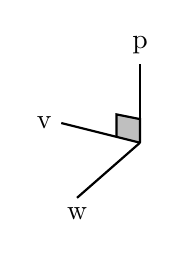
\begin{tikzpicture}
      \coordinate (O) at (0,0);
      \coordinate (P) at (0,1);
      \coordinate (V) at (-1,0.25);
      \coordinate (W) at (-0.8,-0.7);

      \draw[thick,fill=lightgray] (-0.3,0.08) -- (-0.3,0.36) -- (0.0,0.3) -- (0,0);

      \draw[thick] (O) -- (P);
      \draw[thick] (V) -- (O);
      \draw[thick] (W) -- (O);

      \node[above] at (P) {p};
      \node[left] at (V) {v};
      \node[below] at (W) {w};
    \end{tikzpicture}}
  \caption{Cross product of two vectors $v$ and $w$, resulting in a vector $p$ orthogonal to $v$ and $w$.}
  \label{fig:cross-product}
\end{figure}

\subsubsection{Matrices}

Matrices are used to represent transformations in computer graphics. A matrix can be defined in row-major order as:

\begin{equation}
  \label{eqn:matrix}
  M = \begin{bmatrix} M_{1,1} & M_{1,2} \\ M_{2,1} & M_{2,2} \end{bmatrix} = \begin{bmatrix} a & b \\ c & d \end{bmatrix}
\end{equation}

\subsubsection{Ray}

A ray can be defined as $r = (Q, d)$, where $Q$ is the origin vertex of the ray and $d$ is the direction.

\subsubsection{Triangle}

A triangle can be defined as $t = (Q, u, v)$, where $Q$ is the position of the triangle and $u$ and $v$ are vectors defining the triangle. See \autoref{fig:q-u-v-parameterization} for a visual representation.

\begin{figure}[H]
  \centering
  \tikzsetnextfilename{q-u-v-parameterization}
  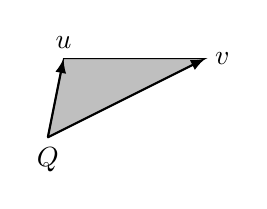
\begin{tikzpicture}
    \draw[fill=lightgray]   (0,0) coordinate[label=below:$Q$] (q) --
    (2,1) coordinate[label=right:$v$] (v) --
    (0.2,1) coordinate[label=above:$u$] (u) -- cycle;

    \draw[-latex, thick] (q) -- (u);
    \draw[-latex, thick] (q) -- (v);
  \end{tikzpicture}
  \caption{Triangle defined using three vertices, $Q$ as the position and $u$,$v$ as direction vectors starting at $Q$.}
  \label{fig:q-u-v-parameterization}
\end{figure}

An alternative way to define a triangle is using three vertices, each in world space. The vertices can be defined as $v_1 = (x_1, y_1, z_1)$, $v_2 = (x_2, y_2, z_2)$ and $v_3 = (x_3, y_3, z_3)$. Converting between the two systems can be done using the following formulas:

\begin{equation}
  \label{eqn:triangle-vertices-to-q-u-v}
  Q = v_1
\end{equation}

\begin{equation}
  \label{eqn:triangle-vertices-to-q-u-v1}
  u = v_2 - v_1
\end{equation}

\begin{equation}
  \label{eqn:triangle-vertices-to-q-u-v2}
  v = v_3 - v_1
\end{equation}

In computer graphics, a triangle has a normal associated with each of its three vertices. Per default, the normal of a vertex is orthogonal to the two adjacent edges of the vertex and can be calculated using the cross product.

\newpage
\subsubsection{Frustum}

The frustum is a geometric shape that defines the camera's view. For a visual representation, see \autoref{fig:camera-frustum}.

\begin{figure}[H]
  \centering
  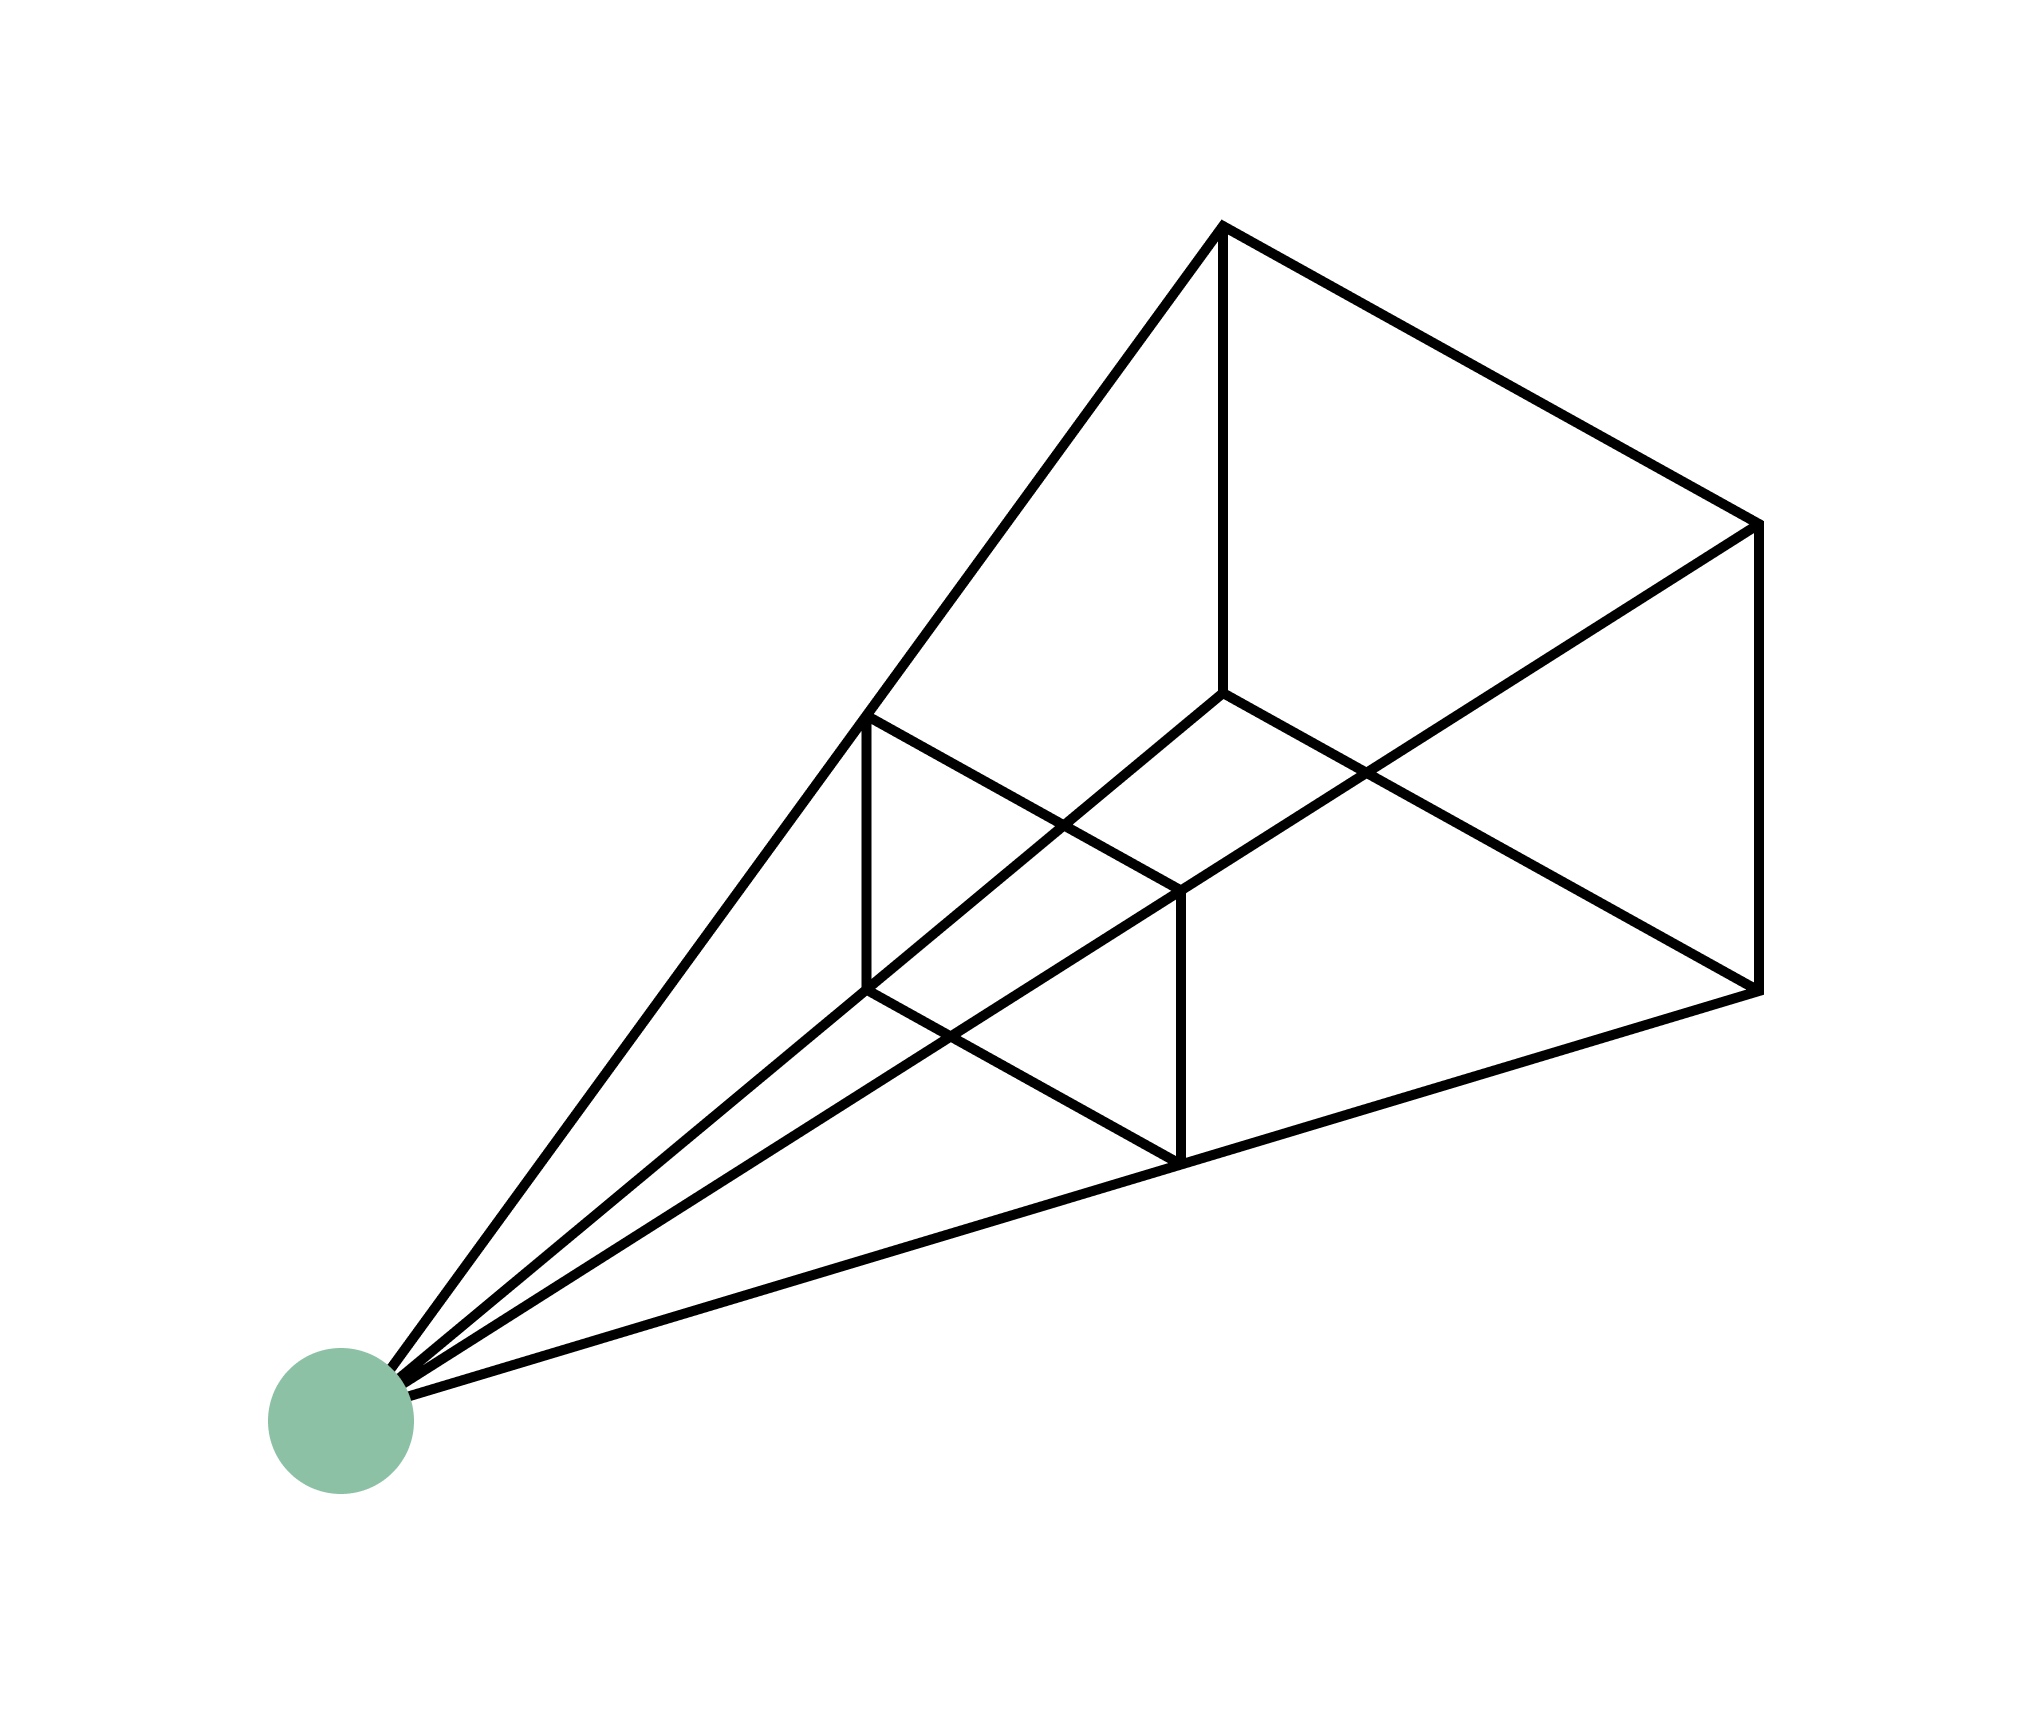
\includegraphics[width=0.25\textwidth]{resources/camera-frustum.png}
  \caption{Frustum shape, the green dot indicates the position of a camera in perspective projection.}
  \label{fig:camera-frustum}
\end{figure}

\subsubsection{Integral}

An integral determines the area under a curve, as visualized in \autoref{fig:integral}. The integral of a function $f(x)$ over an interval $[a, b]$ is defined as:

\begin{equation}
  \label{eqn:integral}
  \int_{a}^{b} f(x) dx
\end{equation}

\begin{figure}[H]
  \centering
  \tikzsetnextfilename{integral}
  \begin{tikzpicture}
    \begin{axis}[
        width=0.4\textwidth,
        xlabel=$x$,
        ylabel=$y$,
        domain=0:2,
        samples=100,
        clip=false,
        axis lines=middle,
        ymin=0, ymax=3.5,
        xmin=0, xmax=2.5,
        xtick={0, 0.5, 1.5},
        ytick={0},
        xticklabels={0, $a$, $b$},
      ]
      \addplot[name path=A, rblue, thick] {x/2.5+((x^2)/2)} node[above,pos=1] {$f(x)$};
      \path[name path=B] (axis cs:0,0) -- (axis cs:2,0);
      \addplot[rblue!50, opacity=0.5] fill between[of=A and B, soft clip={domain=0.5:1.5}];

      % otherwise the left axis will be cropped, even if clip is set to false
      \addplot[draw=none] coordinates {(-0.1,0)};
    \end{axis}
  \end{tikzpicture}
  \caption{Visualization of integral, the area under the curve $f(x)$ between $a$ and $b$.}
  \label{fig:integral}
\end{figure}

In order to take an integral over a different domain $S$, which may represent a set of vectors representing directions, the integral can be defined as:

\begin{equation}
  \label{eqn:integral-domain}
  \int_{S} f(x) dx
\end{equation}

\newpage
\subsubsection{Probability Theory}
\label{sec:probabilityTheory}

Variance is a measure of dispersion, defining how large the difference between the average and the individual values in a set of numbers is. It is calculated as the average of the squared differences from the mean. The variance of a set of numbers $x_1, x_2, ..., x_n$ is defined as:

\begin{equation}
  \label{eqn:variance}
  \sigma^2 = \frac{1}{n} \sum_{i=1}^{n} (x_i - \mu)^2
\end{equation}

where $\mu$ is the mean of the set of numbers.

The standard deviation ($\sigma$) is the square root of the variance ($\sigma^2$). It is a measure of the dispersion of a set of numbers and can be used to determine a confidence interval. This interval is a range of values that has a certain probability of containing the value. High variance leads to a wide confidence interval, which indicates that the data is spread out. The confidence interval ($CI$) as a $\pm$ margin of error deviation from the mean is then defined as:

\begin{equation}
  \label{eqn:confidence-interval}
  CI = \mu \pm z \frac{\sigma}{\sqrt{n}}
\end{equation}

where $z$ is the z-score of the desired confidence level, for example, $1.96$ for a $95\%$ confidence interval, and $n$ is the number of samples.

This can be used to assess the quality and reliability of measurements such as required for benchmarking.

Another important concept is the probability density function (\gls{PDF}). It describes the likelihood of a random variable to take on a specific value. It is related to the cumulative distribution function (\gls{CDF}), which describes the probability that the random variable will be less than or equal to a specific value. The \gls{CDF} can be expressed as the integral of its \gls{PDF}. See \autoref{fig:probability-theory} for a visualization.

\begin{figure}[H]
  \begin{subfigure}[b]{0.4\textwidth}
    \centering
    \tikzsetnextfilename{pdf-theory}
    \begin{tikzpicture}
      \begin{axis}[
          width=6cm,
          axis lines = left,
          xlabel = $x$,
          ylabel = $f(x)$,
          domain=-4:4,
          samples=100,
          enlargelimits=upper,
          xtick=\empty,
          ytick=\empty,
        ]
        \addplot[
          smooth,
          ultra thick,
          rblue,
        ] {1/(sqrt(2*pi))*exp(-x^2/2)};
      \end{axis}
    \end{tikzpicture}
    \caption{\gls{PDF} visualized}
    \label{fig:pdf-theory}
  \end{subfigure}
  \hfill
  \begin{subfigure}[b]{0.4\textwidth}
    \centering
    \tikzsetnextfilename{cdf-theory}
    \begin{tikzpicture}
      \begin{axis}[
          width=6cm,
          axis lines = left,
          xlabel = $x$,
          ylabel = $F(x)$,
          samples=100,
          enlargelimits=upper,
          xtick=\empty,
          ytick={0,1},
        ]
        \addplot[
          smooth,
          ultra thick,
          rgreen,
        ] {1/(1+e^(-1.65451*x))}; % See https://mathoverflow.net/q/273754
      \end{axis}
    \end{tikzpicture}
    \caption{\gls{CDF} visualized}
    \label{fig:cdf-theory}
  \end{subfigure}
  \caption{\gls{PDF} and \gls{CDF} of normal distribution visualized}
  \label{fig:probability-theory}
\end{figure}

\subsubsection{Bachmann-Landau Notation}

The Bachmann-Landau notation, or more specifically, the Big O notation, is used to describe the behavior of a function as the input size grows. The notation is used to describe the upper bound of a function. For example, if a function $f(n)$ is $O(n^2)$, it means that the function grows at most quadratically with the input size $n$. The Big O notation is used to describe the growth of algorithms in terms of run time or space requirements. See \autoref{fig:big-o-visualization} for a visualization.

\begin{figure}[H]
  \centering
  \tikzsetnextfilename{big-o-visualization}
  \begin{tikzpicture}
    \begin{axis}[
        width=0.3\textwidth,
        xlabel=$x$,
        ylabel=$y$,
        domain=0:10,
        samples=100,
        clip=false,
        axis lines=middle,
        ymin=0, ymax=20,
        xmin=0, xmax=11,
        xtick={0},
        ytick={0},
        xticklabels={0},
      ]
      \addplot[rblue, thick] {x} node[above,pos=1] {$O(n)$};
      \addplot[rgreen, thick] {x/1.7} node[right,pos=1] {$f(x)$};
      \addplot[rred, thick, domain=0:5.5] {(x^2)/2} node[above,pos=1] {$g(x)$};

      % otherwise the left axis will be cropped, even if clip is set to false
      \addplot[draw=none] coordinates {(-0.2,0)};
      \addplot[draw=none] coordinates {(0,-0.5)};
    \end{axis}
  \end{tikzpicture}
  \caption{Example of Big O notation, the function $f(x)$ is $O(n)$, but $g(x)$ is not.}
  \label{fig:big-o-visualization}
\end{figure}

\section{Physics}
\label{ch:physics}

In order to generate images using computer graphics, understanding the physics is crucial. More specifically, optics, the study of light and its perception, is essential. The field encompasses topics such as light propagation and optical properties of matter. Maxwell's equations are a set of equations in electromagnetism that describe the behavior of electromagnetic fields. Formulated by James Clerk Maxwell in the 19th century, they provide a mathematical framework for understanding the propagation of electromagnetic waves, including, but not limited to, visible light. Light can be described as a wave or particle, generally known as wave-particle duality. \cite{fowles1989introduction}

In a simplified model, the particles, called photons, are emitted by a light source and travel in straight lines until they hit a surface. The interaction of light with surfaces can be described as a combination of absorption, the law of reflection, and the law of refraction. Absorption is the process of light being converted into other forms of energy, such as heat.

\subsubsection{Reflection}

Reflection is the process of light bouncing off a surface. The angle of incidence equals the angle of reflection, as visualized in \autoref{fig:basic-reflection}. An example of such an effect can be seen when looking at a mirror. This can be described using the law of reflection \cite{fowles1989introduction}:

\begin{equation}
  \label{eqn:law-of-reflection}
  \theta = \theta'
\end{equation}

where $\theta$ is the angle of incidence and $\theta'$ is the angle of reflection.

\begin{figure}[H]
  \centering
  \tikzsetnextfilename{basic-reflection}
  \begin{tikzpicture}
    \coordinate (A) at (0,3);
    \coordinate (AA) at (1,2);
    \coordinate (BB) at (2,1);
    \coordinate (B) at (3,0);
    \coordinate (C) at (6,3);
    \coordinate (BC) at (4,1);
    \coordinate (CB) at (5,2);

    \coordinate (BN) at (3,2);

    \centerarc[thick](B)(90:135:1)
    \node at (2.75,0.7) {$\theta$};

    \centerarc[thick](B)(45:90:1)
    \node at (3.25,0.7) {$\theta'$};

    \draw[dashed, thick] (A) -- (B);
    \draw[-latex, thick] (AA) -- (BB);

    \draw[dashed, thick] (C) -- (B);
    \draw[-latex, thick] (BC) -- (CB);

    \draw[darkgray, -latex, thick] (B) --node[midway, left, yshift=0.4cm] {$n$} (BN);

    \fill[rgreen](B) circle (0.1);

    \fill[gray!20] (0,0) rectangle (6,-1);
    \draw[gray!40] (0,0) -- (6,0);
  \end{tikzpicture}
  \caption{Reflection of light when hitting a surface.}
  \label{fig:basic-reflection}
\end{figure}

\subsubsection{Refraction}

Refraction is the bending of light when passing through a medium as visualized in \autoref{fig:basic-refraction}. The distortion of objects underwater is an example of such an effect.

\begin{figure}[H]
  \centering
  \tikzsetnextfilename{basic-refraction}
  \begin{tikzpicture}
    \coordinate (A) at (0,3);
    \coordinate (AA) at (1,2);
    \coordinate (BB) at (2,1);
    \coordinate (B) at (3,0);
    \coordinate (Bl) at (3,-3);
    \coordinate (C) at (5,-3);
    \coordinate (BC) at (3.665,-1);
    \coordinate (CB) at (4.335,-2);

    \coordinate (BN) at (3,2);

    \centerarc[thick](B)(90:135:1)
    \node at (2.75,0.7) {$\theta$};

    \draw[darkgray, -latex, thick] (B) --node[midway, left, yshift=0.4cm] {$n$} (BN);

    \draw[dashed, thick] (A) -- (B);
    \draw[-latex, thick] (AA) -- (BB);

    \fill[rgreen](B) circle (0.1);

    \fill[gray!20] (0,0) rectangle (6,-3);

    \draw[darkgray,thick] (Bl) -- (B);

    \centerarc[thick](B)(-56:-90:1)
    \node at (3.2,-0.7) {$\phi$};

    \draw[dashed, thick] (C) -- (B);
    \draw[-latex, thick] (BC) -- (CB);
    \draw[gray!40] (0,0) -- (6,0);
  \end{tikzpicture}
  \caption{Refraction of light when passing through a medium.}
  \label{fig:basic-refraction}
\end{figure}

It can roughly be defined by using Snell's law \cite{fowles1989introduction}:

\begin{equation}
  \label{eqn:snells-law}
  \frac{\sin \theta}{\sin \phi} = n
\end{equation}

or in a more general form:

\begin{equation}
  \label{eqn:snells-law-general}
  n_1 \sin \theta = n_2 \sin \phi
\end{equation}

where $n_1$ and $n_2$ are the refractive indices of the two media, and $\theta$ and $\phi$ are the angles of incidence and refraction, respectively.

Leveraging Snell's law, Fresnel equations can be derived which describe not only the refraction but also the reflection of light when passing through a medium \cite{fowles1989introduction}.

\subsubsection{Material Properties}

Common terminology used to describe the optical properties of materials is helpful in understanding the behavior of light and the challenge of simulating it. Some of the most common terms are:

\begin{itemize}
  \item{Scattering} — the material scatters light. This can be observed in fog or clouds.
  \item{Diffuse Reflection} — light is scattered in all directions, independent of the viewing angle. An example of such a material is paper or chalk. As early as the 18th century, Lambert described the reflection of light on a surface \cite{lambert1760photometria}. Lambertian reflection is still used as a term for diffuse reflection.
  \item{Specular Reflection} — light is reflected in a specific direction. This leads to highlights on the surface.
  \item{Roughness} — defines how smooth the surface of the material is. A rough surface scatters light in many directions, while a smooth surface reflects light in a specific direction.
  \item{Subsurface Scattering} — light penetrates the material and is scattered. An example of such a material is skin or marble.
  \item{Metallic} — the material conducts electricity and typically reflects light in a specific direction, which results in a shiny appearance.
  \item{Dielectric} — materials that do not conduct electricity. These materials are not using metallic reflection and often exhibit a combination of diffuse and specular reflection.
  \item{Absorption} — defines how much of the light a material absorbs. In general, darker colors absorb more light than lighter colors. One prominent example is Vantablack, a highly absorbent material.
  \item{Emission} — the material emits light. An example of such a material is a light bulb or the sun.
  \item{Isotropy} — materials that have the same properties in all directions. An example of such a material is glass or water. Anisotropy, on the other hand, is a property of materials that have different properties in different directions. An example of such a material is wood or brushed metal. In everyday life, polarized sunglasses are an example of the practical application of anisotropy.
  \item{Radiance} — the amount of light a surface emits in a specific direction.
\end{itemize}

\subsubsection{Generalization}
\label{sec:physics-generalization}

Many surfaces combine these effects and need to consider the incident and outgoing directions of light, necessitating a bidirectional reflection model. This model defines where the most significant contribution to overall radiance comes from, commonly called the reflection lobe. Simplified, the main contribution can be visualized per incoming direction using an arc indicating the direction of the most significant contribution. For example, a diffuse surface scatters light in all directions (\autoref{fig:reflection-lobe-intro-diffuse}), while a mirror-like surface reflects light in a specific direction (\autoref{fig:reflection-lobe-intro-specular}). Reflection lobes can be combined to simulate different effects.

\begin{figure}[H]
  \centering
  \begin{subfigure}[t]{0.45\textwidth}
    \centering
    \tikzsetnextfilename{reflection-lobe-intro-diffuse}
    \begin{tikzpicture}
      \coordinate (A) at (0,3);
      \coordinate (AA) at (1,2);
      \coordinate (BB) at (2,1);
      \coordinate (B) at (3,0);

      \draw[dashed, thick] (A) -- (B);
      \draw[-latex, thick] (AA) -- (BB);

      \def\tangentx{3}
      \def\tangenty{0}
      \def\tangentr{3.04}

      \foreach \angle in {-20, -40, -60, -80, -100, -120, -140, -160} {
          \draw[-latex, rgreen] (B) -- ($(\tangentx,\tangenty) - (\angle:\tangentr)$);
        }

      \fill[rgreen] (B) circle (0.1);
      \centerarc[rgreen,ultra thick](B)(0:180:1)

      \fill[gray!20] (0,0) rectangle (6,-1);
      \draw[gray!40] (0,0) -- (6,0);
    \end{tikzpicture}
    \caption{Diffuse surface with light scattering in all directions.}
    \label{fig:reflection-lobe-intro-diffuse}
  \end{subfigure}
  \hfill
  \begin{subfigure}[t]{0.45\textwidth}
    \centering
    \tikzsetnextfilename{reflection-lobe-intro-specular}
    \begin{tikzpicture}
      \coordinate (A) at (0,3);
      \coordinate (AA) at (1,2);
      \coordinate (BB) at (2,1);
      \coordinate (B) at (3,0);

      \coordinate (L) at (4.5,3);

      \draw[dashed, thick] (A) -- (B);
      \draw[-latex, thick] (AA) -- (BB);

      \def\tangentx{3}
      \def\tangenty{0}
      \def\tangentr{3.04}

      \draw[-latex, rgreen] (B) -- ($(\tangentx,\tangenty) - (-131:\tangentr)$);
      \draw[-latex, rgreen] (B) -- ($(\tangentx,\tangenty) - (-135:\tangentr)$);
      \draw[-latex, rgreen] (B) -- ($(\tangentx,\tangenty) - (-139:\tangentr)$);

      \fill[rgreen] (B) circle (0.1);
      \centerarc[rgreen,ultra thick](B)(40:50:1)

      \fill[gray!20] (0,0) rectangle (6,-1);
      \draw[gray!40] (0,0) -- (6,0);
    \end{tikzpicture}
    \caption{Mirror-like surface with a small reflection lobe.}
    \label{fig:reflection-lobe-intro-specular}
  \end{subfigure}
  \caption{Bidirectional reflection models for two different types of surfaces with green arc indicating the direction of the largest contribution to reflection.}
  \label{fig:reflection-lobe-intro}
\end{figure}

\section{Computer Graphics}
\label{ch:computerGraphics}

This section provides an overview of computer graphics, including its history, key concepts, and applications.

Since the early days of computing, researchers have explored ways to process visual information using computers. While the field also encompasses aspects such as image processing or two-dimensional graphics, this thesis mainly focuses on three-dimensional computer graphics. Topics such as animation and geometry processing will not be covered. The main topics for this thesis are geometry representation, rendering, and shading.

A 3D scene can be defined as a collection of objects in a three-dimensional space. The basic building blocks of a 3D scene are the triangles, which form the geometry of the objects. The goal is to get this abstract representation of a scene onto a 2D screen. However, to obtain photorealistic images, the rendering needs to consider advanced lighting effects.

\subsection{Global Illumination}

Research to render advanced lighting effects using computer graphics was conducted as early as the 1960s. One of the earliest papers describing approaches to render shadow casting was written in 1968 by Appel \cite{appel1968shading}. In order to describe the phenomena, a more advanced shading model was required. To describe these phenomena, the term global illumination was coined by Whitted in 1979 \cite{whittedGlobalIllumination}. It describes a complete shading model that simulates real lighting and reflection as accurately as possible \cite{whitted2020OriginsOfGlobalIllumination}.

While global illumination commonly refers to a subset of effects, the term is used here to encompass a wide range of effects. Simulating real lighting includes effects such as:

\begin{itemize}
  \item{Shadow Casting} — The absence of light as obstructed by other objects.
  \item{Reflection}
  \item{Color Bleeding} — Special type of reflection where a surface is colored by reflection of colored light.
  \item{Ambient Occlusion} — Special type of shadow casting, where light transport as impacted by nearby objects is considered. This is frequently encountered on objects with complex topology.
  \item{Refraction}
  \item{Caustics} — Effect produced by either reflection or refraction of light.
\end{itemize}

The importance of achieving these effects depends on the use case. For the use case of this thesis, shadows and reflections are pivotal for the realism and perceived quality of the images. Refraction and caustics were not encountered in the use case of this thesis and are, therefore, not covered in detail.

\autoref{fig:global-illumination-demo} depicts the most notable effects and their absence. The scene consists of a floor with a white diffuse material, two walls with a red diffuse material, and a sphere with specular reflection. The sphere casts a shadow onto the floor, the walls are reflected onto the sphere, the prominent red color bleeds onto the white floor.

\begin{figure}[H]
  \centering
  \hspace*{1.8cm}
  \begin{subfigure}[b]{0.3\textwidth}
    \centering
    
\includegraphics[width=\textwidth]{resources/global-illumination-demonstration-negative.png}
    \caption{No global illumination.}
    \label{fig:global-illumination-demo-bad}
  \end{subfigure}
  \hfill
  \begin{subfigure}[b]{0.3\textwidth}
    \centering
    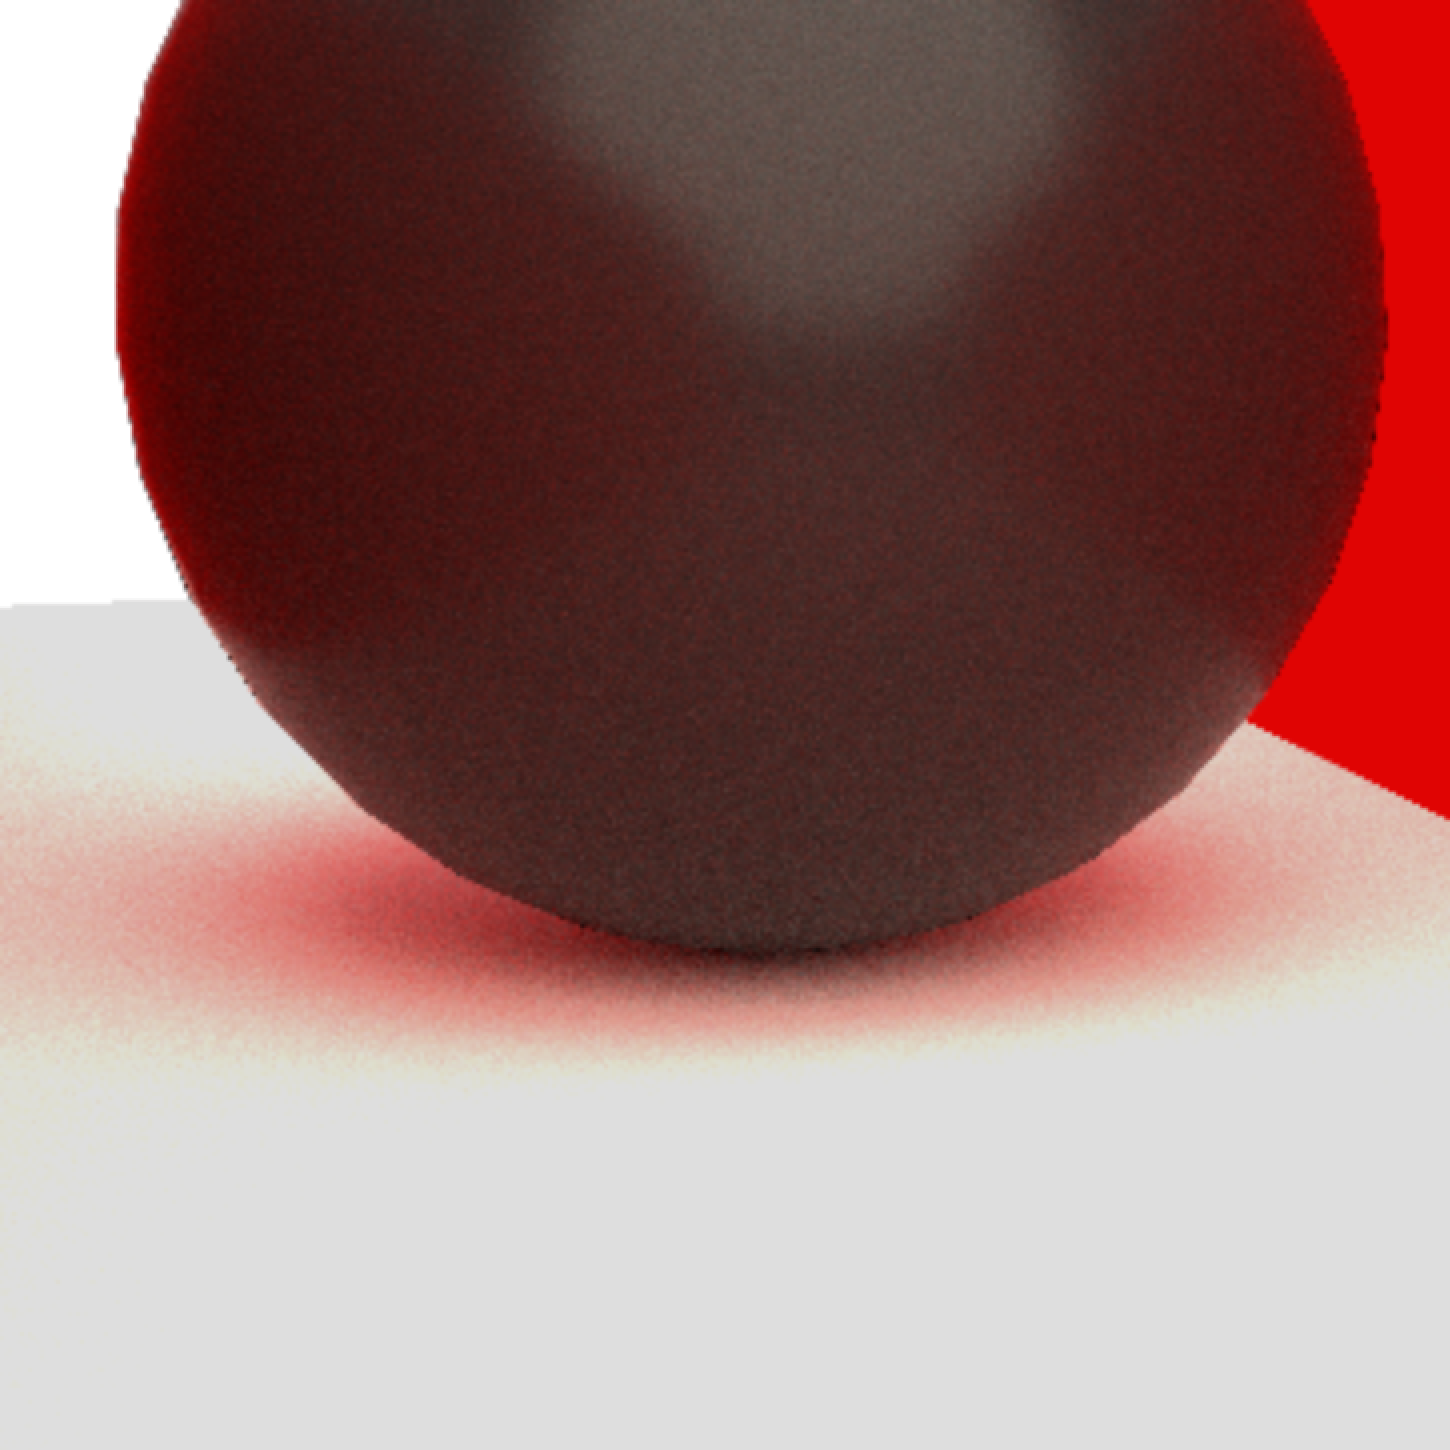
\includegraphics[width=\textwidth]{resources/global-illumination-demonstration.png}
    \caption{With global illumination.}
    \label{fig:global-illumination-demo-good}
  \end{subfigure}
  \hspace*{1.8cm}
  \caption{Side-by-side demonstration of different kinds of global illumination effects.}
  \label{fig:global-illumination-demo}
\end{figure}

\subsection{Rasterization}
\label{ch:rasterizationTheory}

Different rendering approaches have been developed to visualize 3D scenes using a computer. Two of the most common approaches are rasterization and ray tracing. Rasterization will be described in more detail in this section; ray tracing will be discussed in the next section.

Rasterization is a rendering technique that maps the geometry of a 3D scene onto a 2D plane. It is well-suited for real-time rendering due to its efficiency. The rasterization process can be broken down into multiple steps, commonly referred to as the graphics pipeline. The stages of the pipeline are shown in \autoref{fig:graphics-pipeline}.

\begin{figure}[H]
  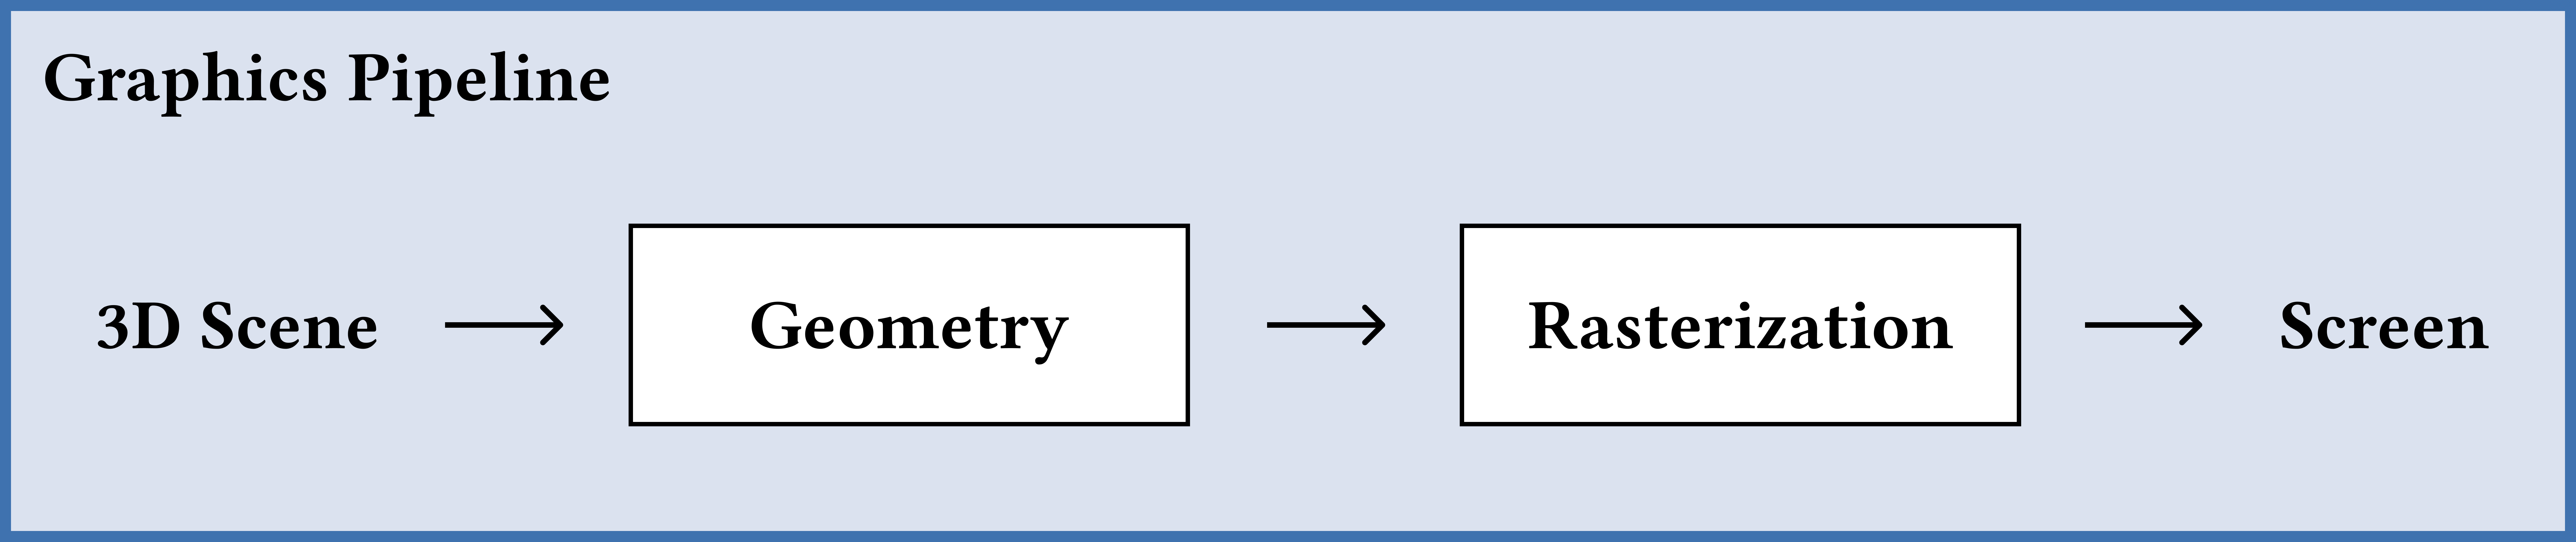
\includegraphics[width=\columnwidth]{resources/graphics-pipeline.png}
  \caption{The main steps of the graphics pipeline used for rasterization.}
  \label{fig:graphics-pipeline}
\end{figure}

As a pre-requisite, the 3D scene is defined. The scene consists of vertices grouped into triangles, forming the geometry. The geometry stage iterates over all triangles and uses the camera configuration to perform view projection as described in \autoref{sec:viewProjection}, changing the position of the vertices to the camera's perspective. The rasterization stage converts the continuous geometry into discrete fragments. When having overlapping triangles, the depth buffer is used to determine which fragment is closer to the camera and, therefore, visible. The fragment processing determines the color of every pixel. Finally, the frame buffer is output to the screen.

One of the main limitations is the lack of support for global illumination. For example, shadows are generally not cast, reflections are not visible, color bleeding is not considered, and ambient occlusion is not simulated.

\subsubsection{Advanced Techniques}

To address these limitations, the graphics pipeline can be extended with additional steps such as post-processing effects or advanced rendering techniques. Various methods have been developed, including pre-baked shadow, environment \cite{greene1986environment} and light maps; screen space reflections (SSR) \cite{screenSpaceReflectionsStackowiak}; screen space ambient occlusion (SSAO) \cite{bavoil2008ssao}; and screen space directional occlusion (SSDO) \cite{ritschel2009ssdo}.

\paragraph{Environment Maps}

Environment maps can be used to simulate reflections. The technique uses a texture that is mapped to the environment of the scene and is used to simulate reflections. Environment maps not support reflections occurring dynamically in the scene, such as self-reflections or reflections of nearby objects.

\paragraph{Shadow Maps}

Shadow maps are employed to store shadow information for a scene based on the available light sources. These shadows are pregenerated, before being employed in the rendering process. While this technique is suitable for static scenes, there are limitations in dynamic lighting situations and scenes where different components of an assembly cast shadow on one another.

\paragraph{Screen Space Methods}

Screen space methods operate on the rendered image. Their input varies, but they frequently rely on the depth buffer, surface normals, and the rendered image. The main drawback of these methods is their limitation to the information available in the rendered image. Occlusion or out-of-view objects are not considered.

\paragraph{Multi-pass Rendering}

Multi-pass rendering is a technique that, among other effects, can be used to simulate reflections. Instead of rendering the scene in a single pass, the scene is rendered multiple times with different configurations. For example, to simulate reflections, one first renders from the perspective of the reflective object and then renders a second pass from the camera while leveraging the first pass as a texture. When having multiple reflective objects, the technique can become computationally expensive.

\paragraph{Conclusion}

Each of these methods addresses only a specific limitation of rasterization. Some of them only partially alleviate the issue. These approaches induce complexity, may need to be computed at the assembly level, and can be computationally expensive. An alternative technique that resembles reality more closely could alleviate these issues: ray tracing.

\subsection{Ray Tracing}
\label{ch:rayTracingTheory}

Ray tracing is a rendering technique which simulates light transport in a scene. Forward ray tracing traces the photons, commonly referred to as rays, from the light source onto the objects. These algorithms are inefficient as most rays do not contribute to the illumination visible in the viewport. Therefore, backward ray tracing is more commonly used. Rays are cast from the camera into the scene, and the object's color with which the ray intersects is computed. In contrast to a rasterizer, which iterates over the triangles of the scene, ray tracing iterates over the pixels of the image. For each pixel, a ray is cast into the scene. By adding additional bounces of the light ray, the technique can simulate global illumination.

Early algorithms were based on recursive ray tracing \cite{whittedGlobalIllumination}. These algorithms determine intersection with geometry and iteratively generate branches as shown in \autoref{fig:recursiveRayTracing}. For each pixel, a primary ray is cast into the scene. When intersecting with a surface, the algorithm considers the light sources and generates secondary rays. These rays are then recursively traced and radiance is calculated until a maximum depth is reached.

\begin{figure}[H]
  \centering
  \begin{subfigure}[t]{0.45\textwidth}
    \centering
    \tikzsetnextfilename{recursive-ray-tracing}
    \begin{tikzpicture}
      \coordinate (A) at (0,2);
      \coordinate (AB) at (0.5,1.5);
      \coordinate (BA) at (1.5,0.5);
      \coordinate (B) at (2,0);
      \coordinate (BBl) at (2,-0.5);
      \coordinate (BlB) at (2,-1.0);
      \coordinate (Bl) at (2,-1.5);
      \coordinate (C) at (4,2);
      \coordinate (BC) at (2.5,0.5);
      \coordinate (CB) at (3.5,1.5);
      \coordinate (CCl) at (4,2.5);
      \coordinate (ClC) at (4,3);
      \coordinate (Cl) at (4,3.5);
      \coordinate (D) at (6,0);
      \coordinate (CD) at (4.5,1.5);
      \coordinate (DC) at (5.5,0.5);


      \fill[gray!20] (0,0) rectangle (6,-1.5);
      \fill[gray!20] (2,2) rectangle (6,3.5);
      \draw[gray!40] (0,0) -- (6,0);
      \draw[gray!40] (2,2) -- (6,2);
      \draw[gray!40] (2,2) -- (2,3.5);

      \draw[dashed, thick] (A) -- node[midway, right] {$i$} (B);
      \draw[-latex, thick] (AB) -- (BA);

      \draw[dashed, thick] (B) -- node[midway, right] {$t_1$} (Bl);
      \draw[-latex, thick] (BBl) -- (BlB);

      \draw[dashed, thick] (B) -- node[midway, right] {$s_1$} (C);
      \draw[-latex, thick] (BC) -- (CB);

      \draw[dashed, thick] (C) -- node[midway, right] {$t_2$} (Cl);
      \draw[-latex, thick] (CCl) -- (ClC);

      \draw[dashed, thick] (C) -- node[midway, right] {$s_2$} (D);
      \draw[-latex, thick] (CD) -- (DC);


      \fill[rgray] (B) circle (0.1);
      \fill[rgray] (C) circle (0.1);
    \end{tikzpicture}
    \caption{Incident ray hitting a surface generating two branches, $s_1$ and $t_1$.}
    \label{fig:recursiveVisualized}
  \end{subfigure}
  \hfill
  \begin{subfigure}[t]{0.45\textwidth}
    \centering
    \tikzsetnextfilename{recursive-tree}
    \begin{tikzpicture}
      \coordinate (A0) at (0,1);
      \coordinate (A0A) at (0,0.75);
      \coordinate (AA0) at (0,0.25);
      \coordinate (A) at (0,0);
      \coordinate (AB1) at (-0.25, -0.25);
      \coordinate (B1A) at (-0.75, -0.75);
      \coordinate (B1) at (-1,-1);
      \coordinate (AB2) at (0.25, -0.25);
      \coordinate (B2A) at (0.75, -0.75);
      \coordinate (B2) at (1,-1);

      \coordinate (B1B11) at (-1.25, -1.25);
      \coordinate (B11B1) at (-1.75, -1.75);
      \coordinate (B11) at (-2,-2);
      \coordinate (B1B12) at (-0.75, -1.25);
      \coordinate (B12B1) at (-0.25, -1.75);
      \coordinate (B12) at (0,-2);

      \draw[dashed, thick] (A0) -- node[midway, right] {$i$} (A);
      \draw[-latex, thick] (A0A) -- (AA0);
      \draw[dashed, thick] (A) -- node[midway, right] {$s_1$} (B1);
      \draw[-latex, thick] (AB1) -- (B1A);
      \draw[dashed, thick] (B1) -- node[midway, right] {$s_2$} (B11);
      \draw[-latex, thick] (B1B11) -- (B11B1);
      \draw[dashed, thick] (B1) -- node[midway, right] {$t_2$} (B12);
      \draw[-latex, thick] (B1B12) -- (B12B1);
      \draw[dashed, thick] (A) -- node[midway, right] {$t_1$} (B2);
      \draw[-latex, thick] (AB2) -- (B2A);

      \fill[rgray] (A) circle (0.1);
      \fill[rgray] (B1) circle (0.1);
    \end{tikzpicture}
    \caption{Recursive ray tracing visualized as a tree structure.}
    \label{fig:recursiveTree}
  \end{subfigure}
  \caption{Recursive ray tracing as described by Whitted \cite{whittedGlobalIllumination}.}
  \label{fig:recursiveRayTracing}
\end{figure}

Due to the computational complexity of these early algorithms, ray tracing was not widely adopted until the 1980s. During these years, one of the main contributions was the introduction of the rendering equation by Kajiya in 1986 in a paper that also coined the term path tracing. Generally, path tracing can be seen as a Monte Carlo integration of the rendering equation, which is defined as:

\begin{equation}
  \label{eqn:rendering-equation}
  I(x, x') = g(x, x') [\epsilon(x, x') + \int_{S} p(x, x', x'')I(x', x'')dx'']
\end{equation}

where $I(x, x')$ is the radiance from point $x$ to point $x'$. $x$ for example being the camera position, and $x'$ the intersected object. $g(x, x')$ is a geometry term determining how much light is transmitted. This depends on the distance and possibly occlusions such as transparent surfaces. $\epsilon(x, x')$ is the emitted radiance, generally used for light sources. The integral term is taken over $S$ = $\cup S_i$ which is the union of all surfaces. $p(x, x', x'')$ is the bidirectional reflection function, which describes how light from all possible directions $x''$ is reflected at the surface. \cite{kajiya1986rendering}

Further research into light transport techniques such as bidirectional light transport or Metropolis light transport has been conducted in the 1990s \cite{veachMonteCarloLightTransport}. Concrete techniques will be described in the next section.

\newpage
\subsubsection{Monte Carlo Integration}
\label{sec:monte-carlo-integration-sampling}

Monte Carlo integration is a statistical technique to approximate the solution of an integral numerically for cases where the integral cannot be solved analytically. At the core of the integration lies an estimator ($G$), which can be defined as:

\begin{equation}
  G = \frac{1}{M}\sum_{i=1}^M g(X_i)
  \label{eq:monteCarlo}
\end{equation}

where $G$ is the estimate of the solution, $g$ is the function to be approximated, and $X_i$ is the random sample. Taking $M$ samples and averaging the results provides an estimate of the solution. \cite{kalos2009monte}

In the context of ray tracing, a path tracing algorithm leverages Monte Carlo integration to approximate the rendering equation, as defined in \autoref{eqn:rendering-equation}. The radiance of a pixel can be approximated by iteratively casting rays into the scene and averaging the results.

While Monte Carlo integration is a powerful technique, it heavily relies on the quality of the estimator that is employed. Using importance sampling can improve the rate of convergence. Importance sampling is a technique that leverages a proposal \gls{PDF}, different from the target \gls{PDF}, to estimate the expected value of a target function. By sampling more frequently in regions where the function has a higher value, the variance of the estimator can be reduced. In order to account for the probability distribution and prevent bias in the estimator, the estimator can be defined as:

\begin{equation}
  G = \frac{1}{M}\sum_{i=1}^M \frac{g(X_i)}{p(X_i)}
  \label{eq:importanceSampling}
\end{equation}

where $p(X_i)$ is the proposal \gls{PDF} \cite{Pharr_Physically_Based_Rendering_2023}.

To do the sampling, different strategies can be considered. For example, one can use the material properties to determine where to cast the rays. A highly reflective surface, such as a mirror, will apply the law of reflection, while a diffuse surface will scatter the rays in all directions. This strategy yields solid results for scenes with large light sources and reflective surfaces, as illustrated in \autoref{fig:material-sampling-good}. However, for scenes with small light sources and diffuse surfaces, the strategy can lead to high variance due to rays that miss the emissive surfaces most of the time, as shown in \autoref{fig:material-sampling-bad}. The variance is visible to the human eye as noise in the image.

\begin{figure}[H]
  \centering
  \begin{subfigure}[t]{0.45\textwidth}
    \centering
    \tikzsetnextfilename{material-sampling-bad}
    \begin{tikzpicture}
      \coordinate (A) at (0,3);
      \coordinate (AA) at (1,2);
      \coordinate (BB) at (2,1);
      \coordinate (B) at (3,0);

      \coordinate (L) at (4.66,2.9);

      \draw[dashed, thick] (A) -- (B);
      \draw[-latex, thick] (AA) -- (BB);

      \def\radius{0.3}

      \def\tangentx{3}
      \def\tangenty{0}
      \def\tangentr{3.04}

      \shade[ball color=yellow!50, opacity=0.3] (L) circle (\radius);
      \draw[yellow!50!black] (L) circle (\radius);

      \foreach \angle in {-20, -40, -60, -80, -100, -140, -160} {
          \draw[-latex, rred] (B) -- ($(\tangentx,\tangenty) - (\angle:\tangentr)$);
        }
      \draw[-latex, rgreen] (B) -- ($(\tangentx,\tangenty) - (-120:\tangentr)$);

      \fill[rgreen] (B) circle (0.1);
      \centerarc[rgreen,ultra thick](B)(0:180:1)

      \fill[gray!20] (0,0) rectangle (6,-1);
      \draw[gray!40] (0,0) -- (6,0);
    \end{tikzpicture}
    \caption{Ray hitting a diffuse surface with bad-performing material sampling.}
    \label{fig:material-sampling-bad}
  \end{subfigure}
  \hfill
  \begin{subfigure}[t]{0.45\textwidth}
    \centering
    \tikzsetnextfilename{material-sampling-good}
    \begin{tikzpicture}
      \coordinate (A) at (0,3);
      \coordinate (AA) at (1,2);
      \coordinate (BB) at (2,1);
      \coordinate (B) at (3,0);

      \coordinate (L) at (4.5,3);

      \draw[dashed, thick] (A) -- (B);
      \draw[-latex, thick] (AA) -- (BB);

      \def\centerx{4.5}
      \def\centery{3}
      \def\radius{1.2}

      \def\tangentx{3}
      \def\tangenty{0}
      \def\tangentr{3.04}

      \shade[ball color=yellow!50, opacity=0.3] (L) circle (\radius);
      \draw[yellow!50!black] (L) circle (\radius);

      \draw[-latex, rgreen] (B) -- ($(\centerx,\centery) - (96:\radius)$);
      \draw[-latex, rgreen] (B) -- ($(\centerx,\centery) - (108:\radius)$);

      \draw[-latex, rred] (B) -- ($(\tangentx,\tangenty) - (-139:\tangentr)$);

      \fill[rgreen] (B) circle (0.1);
      \centerarc[rgreen,ultra thick](B)(40:50:1)

      \fill[gray!20] (0,0) rectangle (6,-1);
      \draw[gray!40] (0,0) -- (6,0);
    \end{tikzpicture}
    \caption{Ray hitting a mirror-like surface with well-performing material sampling.}
    \label{fig:material-sampling-good}
  \end{subfigure}
  \caption{Material sampling strategy weakness and strength}
  \label{fig:material-sampling}
\end{figure}

Light source sampling is an alternative sampling strategy that can alleviate this issue. As shown in \autoref{fig:light-sampling-good}, it can significantly reduce the variance of the estimator when having diffuse surfaces and small light sources. Conversely, the strategy can lead to high variance when having large light sources and reflective surfaces, as shown in \autoref{fig:light-sampling-bad}.

\begin{figure}[H]
  \centering
  \begin{subfigure}[t]{0.45\textwidth}
    \centering
    \tikzsetnextfilename{light-sampling-bad}
    \begin{tikzpicture}
      \coordinate (A) at (0,3);
      \coordinate (AA) at (1,2);
      \coordinate (BB) at (2,1);
      \coordinate (B) at (3,0);

      \coordinate (L) at (4.5,3);

      \draw[dashed, thick] (A) -- (B);
      \draw[-latex, thick] (AA) -- (BB);

      \def\centerx{4.5}
      \def\centery{3}
      \def\radius{1.2}

      \shade[ball color=yellow!50, opacity=0.3] (L) circle (\radius);
      \draw[yellow!50!black] (L) circle (\radius);

      \foreach \angle in {0,21.6,43.2,64.8,86.4} {
          \draw[-latex, rred] (B) -- ($(\centerx,\centery) - (\angle:\radius)$);
        }
      \draw[-latex, rgreen] (B) -- ($(\centerx,\centery) - (108:\radius)$);

      \fill[rgreen] (B) circle (0.1);
      \centerarc[rgreen,ultra thick](B)(40:50:1)

      \fill[gray!20] (0,0) rectangle (6,-1);
      \draw[gray!40] (0,0) -- (6,0);
    \end{tikzpicture}
    \caption{Ray hitting a mirror-like surface with bad-performing light source sampling.}
    \label{fig:light-sampling-bad}
  \end{subfigure}
  \hfill
  \begin{subfigure}[t]{0.45\textwidth}
    \centering
    \tikzsetnextfilename{light-sampling-good}
    \begin{tikzpicture}
      \coordinate (A) at (0,3);
      \coordinate (AA) at (1,2);
      \coordinate (BB) at (2,1);
      \coordinate (B) at (3,0);

      \coordinate (L) at (4.5,3);

      \draw[dashed, thick] (A) -- (B);
      \draw[-latex, thick] (AA) -- (BB);

      \def\centerx{4.5}
      \def\centery{3}
      \def\radius{0.3}

      \shade[ball color=yellow!50, opacity=0.3] (L) circle (\radius);
      \draw[yellow!50!black] (L) circle (\radius);

      \foreach \angle in {0,21.6,43.2,64.8,86.4,108} {
          \draw[-latex, rgreen] (B) -- ($(\centerx,\centery) - (\angle:\radius)$);
        }

      \fill[rgreen] (B) circle (0.1);
      \centerarc[rgreen,ultra thick](B)(0:180:1)

      \fill[gray!20] (0,0) rectangle (6,-1);
      \draw[gray!40] (0,0) -- (6,0);
    \end{tikzpicture}
    \caption{Ray hitting a diffuse surface with well-performing light source sampling.}
    \label{fig:light-sampling-good}
  \end{subfigure}
  \caption{Light source sampling strategy weakness and strength}
  \label{fig:light-sampling}
\end{figure}

Both strategies are good candidates under different circumstances. To leverage the benefits of both strategies, Veach extended importance sampling in 1997 by introducing multiple importance sampling (\gls{MIS}) \cite{veachMonteCarloLightTransport}. The idea is to combine multiple sampling strategies to improve the overall estimator. The \gls{MIS} estimator can be defined as:

\begin{equation}
  G = \sum_{h=1}^k \frac{1}{M_h}\sum_{i=1}^{M_h} w_h(X_{h,i})\frac{g(X_{h,i})}{p_h(X_{h,i})}
  \label{eq:multipleImportanceSampling}
\end{equation}

where $w_h$ is the weight of the $h$-th sampling strategy, and $p_h(X_{h,i})$ is the probability distribution of the $h$-th sampling strategy. $w_h$ is the weighting function for the estimator such that the expected value of the estimator is unbiased.

\subsubsection{Russian Roulette}
\label{ch:russianRoulette}

Russian roulette is a technique for improving efficiency by employing probabilistic path termination. It selectively discards paths with low expected radiance contribution. If a path contributes zero radiance to the final image, it can be terminated early without affecting the radiance of the final image. However, if the path has a small but non-zero contribution, discarding it introduces bias into the calculation. Russian roulette solves this by introducing a probability of termination which is inversely proportional to the radiance of the path. Paths with low radiance are more likely to be terminated. Paths that are continued are scaled by the inverse probability of termination. This ensures to account for the bias introduced by the termination.

Mathematically, Russian roulette is commonly formulated as shown in equation \ref{eqn:russian-roulette} \cite{Pharr_Physically_Based_Rendering_2023}.

\begin{equation}
  \label{eqn:russian-roulette}
  I' = \begin{cases} \frac{I-qc}{1-q} & \xi > q \\ c & otherwise \end{cases}
\end{equation}

where $I$ is the radiance of the path, and $q$ is the probability of termination, which can, for instance, be calculated based on the radiance of the path. $\xi$ is a random number between 0 and 1. $c$ is the contribution of the path which is terminated, commonly set to zero. $I'$ is the scaled radiance of the path.

\subsubsection{Intersection Testing}

When casting a ray into the scene, the first step in a ray tracer is to determine where the ray intersects with the geometry of the scene. A brute force approach could determine the intersection distance for each object to the ray and pick the one with the lowest distance. Given the fact, that common objects consist of thousands of triangles ($n$) and require tracing many rays, this approach is not efficient as it would require $O(n)$ intersection tests for each ray.

In order to accelerate the intersection testing, various approaches have been developed.

The bounding volume hierarchy (\gls{BVH}) is an acceleration structure leveraged to reduce the number of ray intersection tests per ray. This method is widely used in ray tracing and has been studied for a long time \cite{rubinWhittedBvh}. The core idea is to group adjacent objects in a bounding volume and structure the hierarchy in a way that all child elements of a node are contained in the bounding volume of the parent node. The nodes, employed for storing the bounding volume are often axis-aligned bounding boxes (\gls{AABB}). This allows for early rejection of branches which are not intersected by the ray. By employing a \gls{BVH}, the number of intersection tests ($n$) can be reduced from $O(n)$ to $O(log(n))$.

An \gls{AABB} ($b$) can be defined as $b = (min, max)$, where $min$ and $max$ are the minimum and maximum vertices of the bounding box. The boxes are then grouped into a hierarchy where the maximum and minimum vertices of the children define the bounding box of the parent, as visualized in \autoref{fig:bvhVisualized}. Good performance of the \gls{BVH} depends on the quality of the hierarchy. A poorly constructed \gls{BVH} can lead to more intersection tests, as shown in \autoref{fig:bvhBad}. This is because intersections need to be tested against all elements: three bounding boxes and four triangles. For a well-constructed \gls{BVH}, the algorithm can reduce the number of intersection tests as visualized in \autoref{fig:bvhGood} by doing the minimum amount of intersection tests: $b_1$, which intersects; $b_2$, which can be discarded after checking; and $b_3$, which necessitates further intersection tests for the two contained triangles. For such a small number of triangles, the overhead of the \gls{BVH} outweighs its benefits. However, for larger scenes, the performance gain is substantial. In the case of well-balanced trees, the number of tests can be halved at each level of the hierarchy.

\begin{figure}[H]
  \centering
  \begin{subfigure}[b]{0.45\textwidth}
    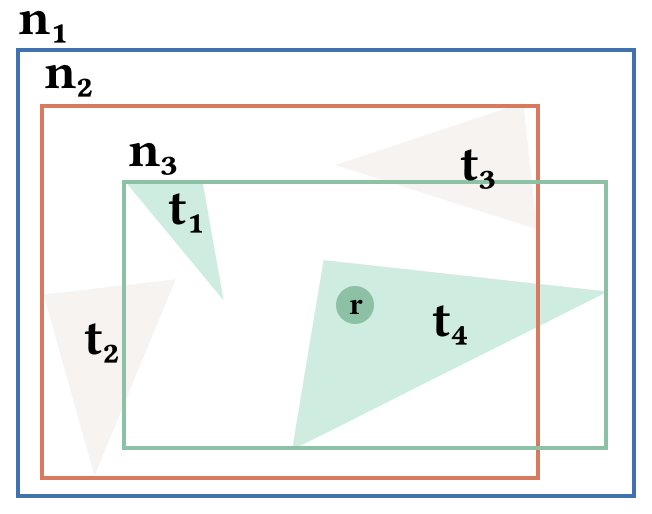
\includegraphics[width=\textwidth]{resources/bvh-bad-visualized.png}
    \caption{Poorly constructed \gls{BVH}, which requires seven intersection tests for $r$, essentially testing against all objects.}
    \label{fig:bvhBad}
  \end{subfigure}
  \hfill
  \begin{subfigure}[b]{0.45\textwidth}
    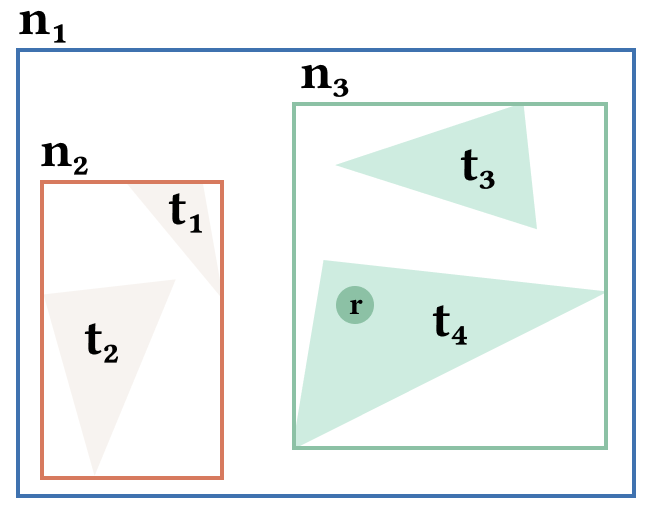
\includegraphics[width=\textwidth]{resources/bvh-good-visualized.png}
    \caption{Well-constructed \gls{BVH}, which reduces the required intersection tests for $r$ to four.}
    \label{fig:bvhGood}
  \end{subfigure}
  \caption{Sample 2D \gls{BVH} visualization, which contains four triangles ($t_1$ to $t_4$) and their corresponding bounding boxes $b_1$ as parent and $b_2$ as well as $b_3$ as the children. $b_1$ is visualized bigger than needed to improve readability. The color of the triangles indicates to which bounding box they belong. $r$ indicates the ray to be tested for intersection.}
  \label{fig:bvhVisualized}
\end{figure}

After the intersection tests on the \gls{AABB}, the actual intersection tests with the triangles contained in the bounding box need to be performed by using an algorithm such as the Möller-Trumbore algorithm \cite{mollerTrumboreFastRayTriangleIntersection}.

\subsubsection{Production Ray Tracing}

Early ray tracing applications were primarily for research purposes or special effects in movies. Adoption expanded as computers became more powerful. One of the first widely used ray tracing software was \fGls{POV-Ray}{\e{Persistence of Vision Ray Tracer}, a cross-platform ray tracing renderer officially released in 1991}, released in 1991 \cite{POV_Ray_Documentation}. Blue Moon Rendering Tools (\gls{BMRT}) \cite{bmrt}, a renderer compliant with \fGls{RenderMan}{a software for photorealistic 3D rendering developed by Pixar}, was released in the mid-1990s and was one of the first ray tracing renderers to be used in the industry. In 2003 \gls{RenderMan} included ray tracing capabilities \cite{RenderMan_11_Release_Notes}. Nowadays, ray tracing is widely used in industries such as film, architecture, and automotive.

\subsubsection{Hybrid Approaches}

Ray tracing and rasterization are not mutually exclusive. Hybrid approaches have been developed to leverage a multi-paradigm approach. One such example is PICA PICA, a real-time ray tracing experiment \cite{hybridRenderingBarreBrisebois2019}. The rendering pipeline is split into multiple stages: global illumination, shadow, reflection, and direct lighting. Each stage could be implemented using different techniques, and the strategy could be chosen based on the scene's requirements and the available computational resources.

\subsection{Common Techniques}

While rasterization and ray tracing are inherently different techniques, specific tasks are similar. The following sections discuss common challenges and their differences in rasterization and ray tracing.

\subsubsection{View Projection}
\label{sec:viewProjection}

In order to render an image, a virtual camera needs to be defined. Given a vertex as $p = (x, y, z)$, the view projection is responsible for transforming the vertex into 2D normalized device coordinates. The view projection matrix is a $4x4$ matrix which depends on the projection type and the camera parameters.

Different types of view projection can be used depending on the use case. The most common types are perspective and orthographic projection. Perspective projection simulates the way the human eye perceives the world, objects which are further away appear smaller. On the other hand, orthographic projection does not consider distance, and objects appear the same size regardless of their distance. Orthographic projection is frequently used in domains such as architecture.

These two projection types differ in the view projection matrix. For perspective projection, the following parameters need to be defined:

\begin{description}
  \item[near ($n$)] — The distance from the camera to the near clipping plane.
  \item[far ($f$)] — The distance from the camera to the far clipping plane.
  \item[fov ($\theta$)] — The \textit{field of view} angle, measured in degrees.
  \item[aspect ratio ($r$)] — The ratio of the viewport's width to its height.
\end{description}

The clipping plane parameters $n$ and $f$ are primarily used in rasterization to determine the camera frustum. Objects outside of the frustum are not rendered. Using equations \ref{eqn:perspectiveProjectionHeight} and \ref{eqn:perspectiveProjectionWidth}, the view projection matrix ($P$) for perspective projection is defined in equation \ref{eqn:perspectiveProjectionMatrix}.

\begin{equation}
  \label{eqn:perspectiveProjectionHeight}
  h = 2n \cdot \tan(\frac{\theta}{2} \underbrace{\pi / 180}_{\text{deg to rad}})
\end{equation}

\begin{equation}
  \label{eqn:perspectiveProjectionWidth}
  w = rh
\end{equation}

\begin{equation}
  \label{eqn:perspectiveProjectionMatrix}
  P =
  \begin{bmatrix}
    \frac{2n}{w} & 0            & 0                    & 0                  \\
    0            & \frac{2n}{h} & 0                    & 0                  \\
    0            & 0            & -\frac{f + n}{f - n} & -\frac{2fn}{f - n} \\
    0            & 0            & -1                   & 0
  \end{bmatrix}
\end{equation}

The elements $P_{1,1}$ and $P_{2,2}$ adjust the field of view and therefore the perspective effect. The elements $P_{3,3}$, $P_{3,4}$ and $P_{4,3}$ adjust the near and far clipping planes. In comparison to rasterization, the view projection matrix is used differently in ray tracing. In rasterization, every vertex is transformed by the view projection matrix. In ray tracing, the view projection matrix is only applied to the camera rays.

For orthographic projection, no such projection matrix is required in ray tracing. Instead, parallel rays are cast from the camera grid.

\subsubsection{Random Number Generator}

To simulate light transport, the path tracer needs to pick random directions. Generating a random direction vector, defined as $v = (x, y, z)$, can be achieved by picking three random numbers independent of one another. This is done using a random number generator (\gls{RNG}). In rasterization, the necessity for \gls{RNG} is less common but may still be required for specific effects. There are a variety of \glspl{RNG} available which differ in essential characteristics. Some of the characteristics to consider when choosing a suitable \gls{RNG} are:

\begin{itemize}
  \item{Statistical Quality} — The \gls{RNG} should generate numbers that are statistically random. This means that the numbers should be uniformly distributed and have a low correlation between them.
  \item{Period} — The length of the cycle before the sequence of generated numbers starts to repeat itself.
  \item{Time Performance} — The time it takes to generate a random number. This is influenced by the algorithm as well as the hardware, which may support dedicated instructions.
  \item{Space Usage} — The amount of memory required to store state.
\end{itemize}

Based on the use case, other factors such as prediction difficulty or others such as highlighted by O’Neill \cite{o2014pcg} may be important. Cryptography, for example, requires randomness of the \gls{RNG} to prevent an adversary from predicting secret keys. Options to generate the randomness require additional signals \cite{randomnessCryptography} or may require special hardware, such as \fGls{Lavarand}{a hardware \gls{RNG} based on pictures taken of lava lamps to generate randomness} \cite{cloudflareLavaRand}. Many generators are pseudorandom generators. These generators are deterministic and require a seed to start the sequence. For cryptographically secure generators, the seed must be random.
However, for a path tracer, there is no need for cryptographic security. Instead, it is more important to have high performance and to have a long period to avoid repetition. Therefore, a pseudorandom number generator with non-cryptographically secure seed is used.

One option for such a pseudorandom generator is using Xorshifts, such as described by Marsaglia \cite{marsaglia2003xorshift}. The algorithm can be defined as shown in Figure \ref{code:xorShift}. $x$ is the state of the \gls{RNG} and $a$, $b$ and $c$ are constants which are chosen to achieve good statistical properties. Frequent choices for these constants are $a = 13$, $b = 17$, and $c = 5$.

\begin{figure}[H]
  \begin{lstlisting}[style=wgsl]
x ^= x << a;
x ^= x >> b;
x ^= x << c;
\end{lstlisting}
  \caption{Xorshift \gls{RNG} implementation.}
  \label{code:xorShift}
\end{figure}

The Mersenne Twister \cite{rngMersenneTwister} is an alternative \gls{RNG}. It is a pseudorandom number generator which has a long period and good statistical properties. However, it is slower than Xorshifts \cite{o2014pcg}. More recently, \fGls{PCG}{\e{Permuted Congruential Generator}, a family of random number generators} has been proposed as an alternative to these options. \gls{PCG} is a family of fast generators well-suited for ray tracing use.

\subsubsection{Anti-aliasing}
\label{sec:anti-aliasing}

Aliasing is a common issue in computer graphics. It occurs when the resolution of the screen is not sufficient to represent the scene accurately. One such example is jagged edges on diagonal lines. Anti-aliasing techniques can be employed to reduce the effect. The negative effect of aliasing is demonstrated in \autoref{fig:aliasingA}.

\begin{figure}[H]
  \centering
  \begin{subfigure}[b]{0.45\textwidth}
    
\includegraphics[width=\textwidth]{resources/aliasing.png}
    \caption{Rendering showing aliasing.}
    \label{fig:aliasingA}
  \end{subfigure}
  \hfill
  \begin{subfigure}[b]{0.45\textwidth}
    
\includegraphics[width=\textwidth]{resources/anti-aliasing.png}
    \caption{Rendering with anti-aliasing applied.}
    \label{fig:aliasingB}
  \end{subfigure}
  \caption{The two images show the effect of aliasing and anti-aliasing.}
  \label{fig:aliasing}
\end{figure}

In ray tracing, aliasing can be alleviated by randomizing the direction of the rays for the different samples taken. The result of applying anti-aliasing can be seen in \autoref{fig:aliasingB}.

In rasterization, similar solution strategies can be employed. Supersampling is a common technique that renders the scene at a higher resolution and then downsamples the image by averaging the colors of the pixels. More elaborate techniques, such as deep learning super sampling (DLSS) implemented by NVIDIA \cite{nvidiaDlss}, can be used to further improve the quality of the image.

\subsubsection{Tone Mapping}
\label{sec:toneMappingTheory}

When simulating light transport, the radiance of the scene can exceed the displayable range. Tone mapping is a technique used to map the high dynamic range (\gls{HDR}) input generated by the renderer to a lower dynamic range. The basic idea is to adjust the radiance of the scene to resemble realistic lighting conditions more closely. One common algorithm to do so is the Reinhard tone mapping operator \cite{reinhardToneMapping}. In recent years, special tone mappers have been developed for dedicated use cases. One example is the Khronos \gls{PBR} Neutral Tone Mapper \cite{pbrNeutralToneMapping}, which is designed to work well with rendering true-to-life colors. See \autoref{fig:tone-mapping} for a comparison of tone mapping with and without the Khronos \gls{PBR} Neutral Tone Mapper.

\begin{figure}[H]
  \centering
  \hspace*{2cm}
  \begin{subfigure}[t]{0.3\textwidth}
    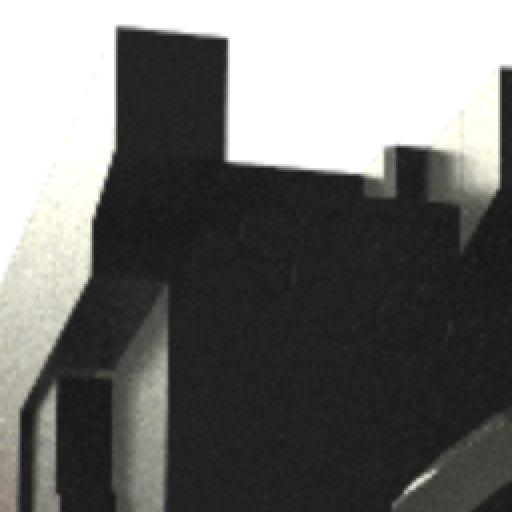
\includegraphics[width=\textwidth]{resources/tonemapping-none.png}
    \caption{Rendering without tone mapping.}
    \label{fig:tone-mapping-none}
  \end{subfigure}
  \hfill
  \begin{subfigure}[t]{0.3\textwidth}
    
\includegraphics[width=\textwidth]{resources/tonemapping-khronos-pbr-neutraltone.png}
    \caption{Rendering using tone mapper.}
    \label{fig:tone-mapping-applied}
  \end{subfigure}
  \hspace*{2cm}
  \caption{Comparison of tone mapping with slight changes in luminance of specular reflection. The upper part is barely visible without tone mapping as it blends into the background due to the high luminance.}
  \label{fig:tone-mapping}
\end{figure}

\section{Computer Graphics Technology}

This section provides an overview of the technology used to render 3D scenes. It will introduce the hardware as well as the software used in the field with a focus on technology relevant for this thesis by introducing \gls{WebGPU} and its core concepts.

\paragraph{Parallel Processing}

Sequential processing is limited in terms of performance. As the amount of data to process grows, the time to process the data grows linearly. Computer graphics exhibits a large number of problems which can be parallelized. In 1966, Flynn introduced a classification system for computer architectures based on the instruction streams and data streams that can be processed in parallel \cite{flynnTaxonomy,flynnTaxonomy2}. Already in 1970, Watkins described an algorithm for computer graphics leveraging a specialized processor for parallel processing \cite{surfaceAlgorithmProcessor}. Further research, such as Chap, a \fGls{SIMD}{\e{Single Instruction, Multiple Data}, a type of parallel processing of data points with a single instruction as defined by Flynn \cite{flynnTaxonomy}} graphics processor proposed in 1984 by Levinthal and Porter as part of Lucasfilm, introduced a special-purpose processor executing a single instruction on multiple data points \cite{chapSIMDgpu}.

\paragraph{GPU}

The first consumer graphics processing unit (\gls{GPU}), the GeForce 256 produced by NVIDIA \cite{evolutionOfGPU}, was developed in the 1990s and extended upon research conducted in the decades prior such as the superworkstations introduced by Silicon Graphics in the 1980s \cite{sigWorkstation}. These workstations were special-purpose computers optimized for computer graphics. The \gls{GPU} on the other hand is a specialized processor that is well-suited for workloads which require parallel processing and can be installed on a standard computer. While \gls{CPU} parallelization on consumer hardware is generally limited to a few cores, modern \glspl{GPU} have thousands of compute units that enable \gls{SIMD} and, more commonly, \fGls{SIMT}{\e{Single Instruction, Multiple Threads}, an extension to \gls{SIMD} which is frequently used on modern \glspl{GPU}} processing. The difference is that \gls{SIMD} operates on a single processor, while \gls{SIMT} operates on multiple processors.

Due to computational complexity, ray tracing techniques have been limited to offline rendering for a long time. Early ray tracers such as \gls{BMRT} were developed, focusing on leveraging the \gls{CPU} for computations. The introduction of \glspl{GPU} has led to further research optimizing speed for ray tracing techniques. One such example of research for a well-established technique is \gls{BVH} construction on the \gls{GPU} \cite{lauterbach2009GPUbvh}. Leveraging \gls{GPU} has been a focus of research and has enabled real-time ray tracing in recent years. Notable developments include reservoir-based spatio-temporal importance resampling (\gls{ReSTIR}) \cite{restir} and subsequent improvements \cite{restirAdvancements,restirGeneralized,restirArea}.

Nowadays, \glspl{GPU} are prevalent in consumer hardware such as smartphones, tablets, laptops, and desktops, and their use case is not limited to computer graphics. \glspl{GPU} are used in various applications, such as machine learning (\gls{ML}), scientific computing, and data processing. Devices that do not have a discrete \gls{GPU} often use an integrated \gls{GPU}, which is part of the \gls{CPU}.

Modern \gls{GPU} hardware offers support for hardware-accelerated ray tracing. Examples include NVIDIA RTX \cite{nvidiaRtxRayTracing}, Apple \gls{Metal} on M3 \cite{appleM3GpuAdvancements}, and others. These examples demonstrate an increasing trend towards hardware-accelerated ray tracing in recent years. However, many devices and \glspl{API}, including \gls{WebGPU}, do not yet support hardware-accelerated ray tracing.

\paragraph{Common Strategies}
\label{sec:commonGpuStrategies}

Specific basic definitions have established themselves as standard practices for graphics \glspl{API}. The term shader describes a program that runs on the \gls{GPU}. The term shader is frequently used in conjunction with different shader types which are used as part of the graphics pipeline in rasterization. The pipeline in its basic form consists of two steps which are executed on the \gls{GPU} in sequence:

\begin{itemize}
  \item{Vertex Shader} — The vertex shader is responsible for transforming the vertices of the geometry into screen space. The output of the vertex shader is a set of vertices which are then rasterized.
  \item{Fragment Shader} — The fragment shader is responsible for determining the color of the fragments that are generated by the rasterizer. It is executed once for each fragment.
\end{itemize}

In addition to this standard graphics pipeline, many \glspl{API} also support custom code which does not need to be used exclusively for rendering. This code can be used for general-purpose computing and is generally referred to as \gls{GPGPU}. The corresponding compute pipeline consists of a single stage where input and output can be configured. Shaders that are used for \gls{GPGPU} are often called compute shaders.

\paragraph{Parallelization Architecture}
\label{sec:parallelization-architecture}

\glspl{GPU} are designed to process data in parallel using \gls{SIMT} architecture. A single instruction is executed on multiple threads, each operating on independent data. The multiple threads are grouped into so-called warps at the hardware level. As only a single instruction is executed per warp, the threads must be synchronized. If one thread in a warp takes a different path, e.g., due to conditional branching, all threads in the warp must wait until the divergent thread completes. This divergence in control flow can lead to performance degradation as demonstrated by Laine et al. \cite{laine2013megakernels}. The performance can be significantly impacted for complex material workflows with highly divergent control flow. One option to address this issue is to use split the shaders from a single monolithic shader, known as a megakernel, into multiple smaller kernels. However, this approach can lead to additional overhead due to the increased coordination efforts, manifested as additional global memory and synchronization mechanisms.

\subsection*{OpenGL}

\gls{OpenGL} is an \gls{API} for rendering 3D graphics. After its introduction in 1992, it was widely adopted. Subsequently, the standard has been ported to other platforms and has been extended with new features. The \gls{API} has its own shading language called OpenGL Shading Language (\gls{GLSL}).

To date, \gls{OpenGL} is still widely used in the industry, but it has been replaced by more modern \glspl{API} in recent years.

\subsection*{Modern Graphics APIs}

While \gls{OpenGL} and derivatives such as \fgls{OpenGL ES}{\e{OpenGL for Embedded Systems}, a subset of \gls{OpenGL} designed for embedded systems like smartphones} have been widely adopted, the introduction of a number of new \glspl{API} has changed the landscape. The standards share an understanding of giving developers more control over the hardware and can be more efficient than \gls{OpenGL}. Modern hardware-accelerated features such as ray tracing are more easily accessible using these new \glspl{API}. Some of the most notable \glspl{API} are:

\begin{itemize}
  \item{\gls{Vulkan}} — Developed by the \fgls{Khronos Group}{a consortium for developing interoperability standards for 3D graphics}, \gls{Vulkan} is a low-level \gls{API} that is supported on a wide range of platforms.
  \item{\gls{Metal}} — Developed by Apple, \gls{Metal} is a low-level \gls{API} that is supported on Apple devices.
  \item{\gls{DirectX 12}} — Developed by Microsoft, DirectX is a collection of \glspl{API} for Microsoft Windows.
\end{itemize}

None of these \glspl{API} are supported in the browser, which makes them unsuitable for the discussed use case.

\subsection*{WebGL}

\gls{WebGL} is a graphics \gls{API} for the web based on \gls{OpenGL ES} 2.0. It was initially released in 2011 and has since been adopted by all major browsers.

\gls{WebGL} is designed to offer a rendering pipeline but does not offer \gls{GPGPU} capabilities. There have been efforts to extend with compute shaders, but efforts by the \gls{Khronos Group} have been halted in favor of focusing on \gls{WebGPU} instead.

Workarounds have been developed to provide \gls{GPGPU} capabilities. The basic idea is to render the output of a fragment shader to a texture and interpret the output as binary data instead of color information. There are libraries such as \texttt{GPU.js} which provide \gls{GPGPU} capabilities using \gls{WebGL}. \texttt{Tensorflow.js}, a library for training and deploying \gls{ML} models, uses similar techniques in the \gls{WebGL} backend.

Since its introduction, \gls{WebGL} has been extended with new features. \gls{WebGL} 2.0, based on \gls{OpenGL ES} 3.0, was released in 2017. Of the major browsers, Safari was the last to support it out of the box in 2021. Since \gls{WebGL} 2.0, no major versions have been released, but new features have been added. This makes it evident that while \gls{WebGL} will remain a viable option for the foreseeable future, \gls{WebGPU} is likely to become the preferred choice in the long term.

\newpage
\subsection*{WebGPU}

\gls{WebGPU} is a new web standard developed by \fGls{W3C}{\e{World Wide Web Consortium}, a non-profit organization dedicated to developing web standards} \cite{webgpuSpecification}. Unlike its predecessor, \gls{WebGL}, it is no longer based on \gls{OpenGL}. One of the main capabilities is support for \gls{GPGPU} by design. While all major browser vendors have announced intent to support \gls{WebGPU}, to date only Chrome has shipped \gls{WebGPU} for general use on desktop as well as mobile.
The standard is still in development and new features are being added.
Common 3D engines such as \gls{Babylon.js}, \gls{Three.js}, \gls{PlayCanvas} and \gls{Unity} have announced support for \gls{WebGPU}.

\subsubsection{Implementations}

Three major implementations of \gls{WebGPU} exist:

\begin{itemize}
  \item{\gls{Dawn}} \cite{dawnImplementation} — Developed by Google, \gls{Dawn} is a C++ library which provides a \gls{WebGPU} implementation. It is used in browsers based on \fGls{Chromium}{a browser engine primarily developed by Google, used in browsers such as Chrome, Edge, and Opera}.
  \item{\gls{wgpu}} \cite{wgpuImplementation} — A Rust library which provides a \gls{WebGPU} implementation. It is used in Firefox and \fGls{Deno}{a JavaScript runtime, alternative to Node.js}.
  \item{\fGls{WebKit}{a browser engine primarily used in Safari} \gls{WebGPU}} \cite{webKitWebGPUImplementation} — Developed by Apple for Safari.
\end{itemize}

As the standard is under active development, there are differences between the implementations and the specification \cite{wgpuStandardDeviation}. However, the implementations are largely compatible thanks to alignment efforts and the extensive conformance test suite \cite{WebGPUConformanceTestSuite}. Generally, these implementations run natively on modern graphics \glspl{API} such as \gls{Vulkan}, \gls{Metal}, and \gls{DirectX 12}. Some also support \gls{OpenGL} and \gls{WebGL} as a fallback.

\subsubsection{Core Concepts}

\gls{WebGPU} is a low-level \gls{API} when compared to \gls{WebGL}. Users get access to the \gls{GPU} via adapters, which abstract the underlying hardware. \gls{WebGPU} fully supports common \gls{GPU} strategies as described in \autoref{sec:commonGpuStrategies}. Most of the commands are then executed on a logical device which is created using the adapter.

For a compute pipeline, one needs to define a pipeline layout that consists of multiple bind group layouts. These define the memory layout of the data that is passed to the \gls{GPU}. The code to be executed is defined in a shader module. The compute pipeline is then created by combining the shader module and the pipeline layout. See \autoref{fig:webgpu-arch} for a visual representation of the core concepts in \gls{WebGPU}. Setting up a graphics pipeline is similar, but two shader module configurations are required.

\begin{figure}[H]
  \centering
  \tikzsetnextfilename{webgpu-arch}
  \begin{tikzpicture}[
      abstract/.style={rectangle, draw=rblue, ultra thick, fill=rbblue, inner sep=0.4cm},
      concrete/.style={rectangle, draw=rgreen, ultra thick, fill=rbgreen, inner sep=0.4cm},
    ]

    \node[abstract] (bgl) {Bind Group Layout};
    \node[concrete, below=of bgl] (bg) {Bind Group};
    \node[concrete, right=of bg] (sm) {Shader Module};
    \node[concrete, right=of sm] (cp) {Compute Pipeline};
    \node[abstract, above=of cp] (pl) {Pipeline Layout};

    \draw[-latex, thick] (bg) -- (bgl);
    \draw[-latex, thick] (pl) -- (bgl);
    \draw[-latex, thick] (cp) -- (sm);
    \draw[-latex, thick] (cp) -- (pl);
  \end{tikzpicture}
  \caption{Core concepts in \gls{WebGPU}, the arrow direction indicates references to. Blue elements are independent of concrete references to data and code, while green elements are concrete references.}
  \label{fig:webgpu-arch}
\end{figure}

Having set up the compute pipeline, one needs to define the bind groups which contain the data. Using a command encoder, the compute pipeline can be dispatched to the \gls{GPU} for execution. The shader describes the expected size of the workgroup, which is a group of threads executed in parallel. The dispatch coordinates how many workgroups are executed. The total number of threads is, therefore, given by the product of the workgroup size and the dispatch size. For a visual representation of a workgroup of size $3x3$ and dispatch size $4x4$, refer to \autoref{fig:gpu-workgroup-layout}.

\begin{figure}[H]
  \centering
  \tikzsetnextfilename{gpu-workgroup-layout}
  \begin{tikzpicture}
    \foreach \x in {0,0.8,1.6,2.4} {
        \foreach \y in {0,0.8,1.6,2.4} {
            \draw[thick, rblue] (\x,\y) rectangle (\x+0.8,\y+0.8);
            % threads within workgroup
            \foreach \i in {0,1,2} {
                \foreach \j in {0,1,2} {
                    \draw[thick, rgreen, fill=rbgreen] (\x+\i*0.25+0.1,\y+\j*0.25+0.1) rectangle (\x+\i*0.25+0.2,\y+\j*0.25+0.2);
                  }
              }
          }
      }
  \end{tikzpicture}
  \caption{\gls{GPU} workgroup layout. Each green square represents a thread within a workgroup. Each blue square represents a workgroup.}
  \label{fig:gpu-workgroup-layout}
\end{figure}

\subsubsection{Shading Language}

\gls{WebGPU} introduces a new shading language called \gls{WebGPU} Shading Language (\gls{WGSL}) \cite{wgslSpecification}. The language is statically typed and supports a variety of data structures required for computer graphics and general-purpose computing.

Every compute pipeline, or render pipeline, requires an entry point, as shown in \autoref{code:computePipelineJs}. This entry point can then be defined as shown in \autoref{code:computePipelineWgsl}. Note that the return type definition is optional for functions.

\begin{figure}[H]
  \begin{lstlisting}[style=JavaScript]
device.createComputePipeline({
  layout: computePipelineLayout,
  compute: {
    module: computeShaderModule,
    entryPoint: "computeMain",
  },
});
  \end{lstlisting}
  \caption{JavaScript code defining the entry point for a compute pipeline.}
  \label{code:computePipelineJs}
\end{figure}

\begin{figure}[H]
  \begin{lstlisting}[style=wgsl]
@compute
@workgroup_size(1, 1, 1)
fn computeMain(@builtin(global_invocation_id) global_id: vec3<u32>) {
  // ...
}
  \end{lstlisting}
  \caption{\gls{WGSL} code defining the entry point for a compute pipeline.}
  \label{code:computePipelineWgsl}
\end{figure}

Attributes such as \texttt{@compute} are used to provide additional information to the compiler. In this case, it denotes the entry point for the compute pipeline and is mandatory as it enables usage of specific attributes such as \texttt{@builtin}, which may only be used on entry points.
In terms of limitations, it is similar to other shading languages. For example, it does not support recursion because cycles are not permitted in declarations. It also does not have features such as an \gls{API} for \gls{RNG}. The shading language is designed for common use cases in computer graphics and general-purpose computing. One example is support for swizzling. Swizzling is a class of operations that facilitate managing vector elements. For example, given a vector \texttt{let v = vec3f(x, y, z)}, the operation \texttt{v.xy} returns a vector \texttt{(x, y)}.

\subsubsection{Data}

Data needs to be transferred between the \gls{CPU} and the \gls{GPU} within bind groups. The core methods to store data are textures and buffers. Textures are optimized for n-dimensional data such as images and offer additional features such as interpolation. Buffers are the primary method to store arbitrary data. Depending on the type of data to be transferred, different buffers can be used:

\begin{itemize}
  \item{Uniforms} — Uniform Buffers are optimized for data which is read-only on the \gls{GPU} and is the same for all vertices or fragments. Such information could be the projection matrix.
  \item{Storage} — Storage Buffers are intended for read-write access on the \gls{GPU}. The size limits of these buffers are higher than for uniform buffers.
  \item{Vertex} — Alternative to storage buffers, intended for vertex data.
  \item{Index} — Buffers which contain indices for the vertices.
\end{itemize}

\subsubsection{Memory Alignment}
\label{ch:memoryAlignmentTheory}

\gls{WGSL} supports \texttt{struct} for defining data structures. However, memory alignment must be considered when passing data between the \gls{CPU} and the \gls{GPU}. Alignment is a constraint, restricting the memory address at which a data structure can be stored. Having strict memory alignment enables the use of more efficient hardware instruction sets or addresses hardware requirements.

Each type in \gls{WGSL} has specific alignment requirements independent of the size. For example, a \texttt{vec3f} has a size of 12 bytes but requires an alignment of 16 bytes. So for a struct definition such as can be seen in \autoref{code:memoryAlignment}, the struct requires 32 bytes of memory to store 20 bytes of data as illustrated in \autoref{fig:memory-alignment}. The excess 12 bytes are used for padding.

\begin{figure}[H]
  \begin{lstlisting}[style=wgsl]
  struct ThreeFields {
    a: f32,
    b: vec3f,
    c: f32
  }
  \end{lstlisting}
  \caption{\gls{WGSL} \texttt{struct} containing three fields of type \texttt{f32} and \texttt{vec3f}.}
  \label{code:memoryAlignment}
\end{figure}

\begin{figure}[H]
  \centering
  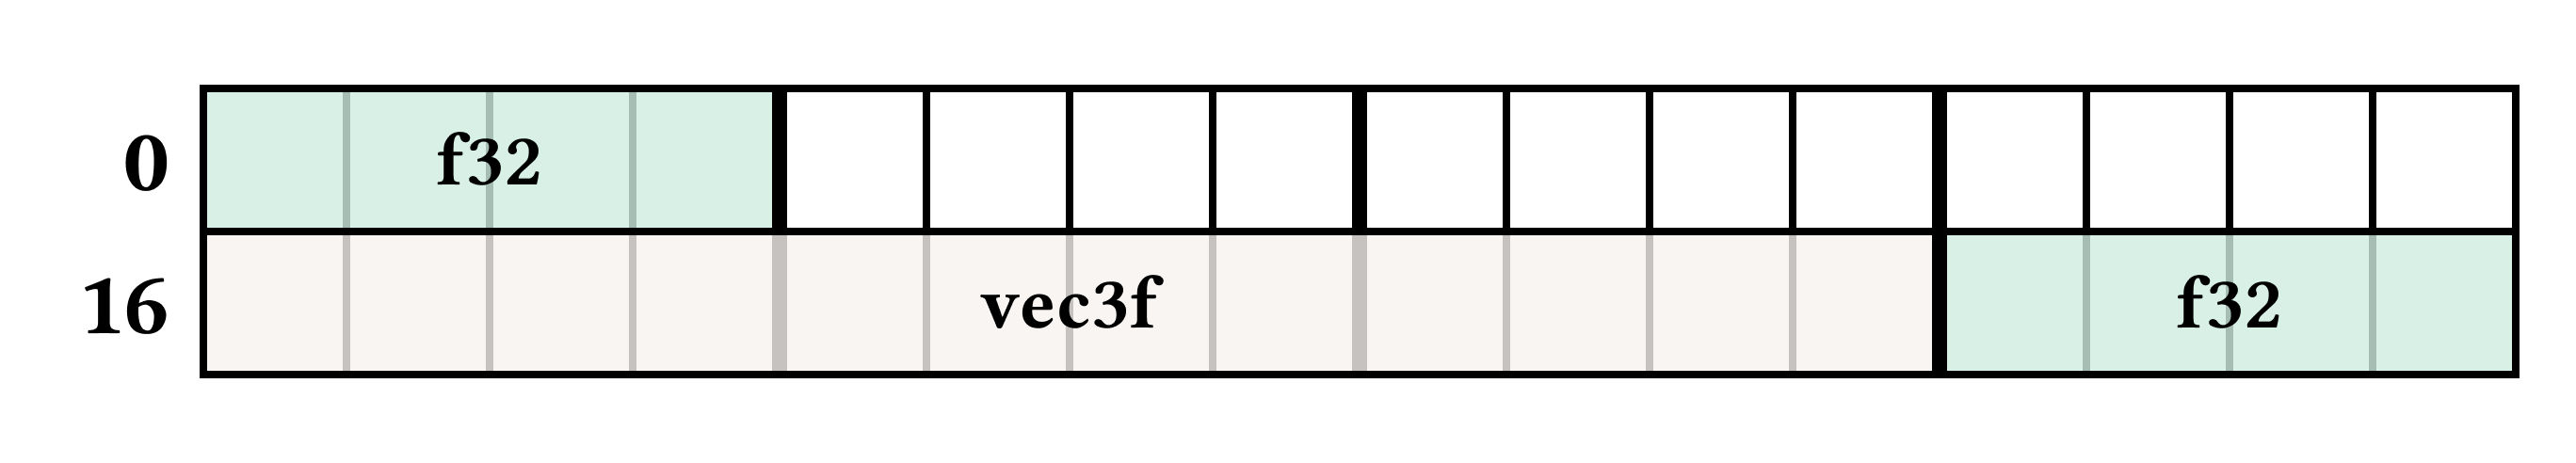
\includegraphics[width=0.8\textwidth]{resources/memory-alignment.png}
  \caption{Memory alignment with padding for struct defined in \autoref{code:memoryAlignment}.}
  \label{fig:memory-alignment}
\end{figure}

Memory alignment is opaque while writing \gls{WGSL} code, but it is relevant when providing data to the \gls{GPU}. The alignment requirements need to be considered when creating buffers. When using JavaScript to create buffers, the standard web \glspl{API} such as \texttt{Float32Array} or \texttt{Uint32Array} can be used to provide data. In order to write data to the \texttt{struct} in \autoref{code:memoryAlignment}, the views can be created as shown in \autoref{code:memoryAlignmentJs}.

\begin{figure}[H]
  \begin{lstlisting}[style=JavaScript]
const ValueBuffer = new ArrayBuffer(32);
const a = new Float32Array(ValueBuffer, 0, 1);
const b = new Float32Array(ValueBuffer, 16, 3);
const c = new Float32Array(ValueBuffer, 28, 1);
  \end{lstlisting}
  \caption{JavaScript code providing views to access the \texttt{struct}.}
  \label{code:memoryAlignmentJs}
\end{figure}

\section{Exchange Formats}

In order to exchange 3D scenes between a multitude of applications, various standardized formats have been developed. These formats are optimized for different use cases depending on the requirements of the application. For this thesis, the focus is on formats well-suited for real-time rendering on the web. In comparison to other use cases, certain aspects are critical on the web. These aspects include:

\begin{itemize}
  \item{Efficiency} — It should be optimized for transmission and loading. While data compression algorithms such as \fGls{gzip}{\e{GNU zip}, a file format and software application for compression and decompression} can alleviate some of the issues during transmission, pure text-based formats are generally less efficient than binary formats.
  \item{Feature Set} — The format should support a wide range of features such as geometry, materials, and scene graphs.
  \item{Extensibility} — The format should be extensible to support additional features.
  \item{Interoperability} — 3D engines and applications should widely support the format.
  \item{Openness} — The format should be open and not proprietary. Additionally, it should be actively maintained.
\end{itemize}

The following section categorizes the formats based on their use case and highlights well-established formats.

\subsection*{General Purpose Formats}

One of the most widely used formats is Wavefront \gls{OBJ}, which was developed in the 1980s. The format is text-based and has basic support for materials and textures via a companion \fGls{MTL}{\e{Material Template Library}, a companion file format to \gls{OBJ} for material definitions} file. However, it lacks support for more advanced features such as animations. Additionally, due to its encoding, it is not well-suited for delivery over the web, compared to more modern alternatives.

Formats such as the proprietary \fGls{FBX}{\e{Filmbox}, a proprietary 3D exchange format nowadays managed by Autodesk} by Autodesk, established in 2006, can address the shortcomings in terms of feature set. A wide range of applications supports the format. However, one of the main disadvantages is the proprietary nature of the format, which can make it challenging to integrate in applications which do not have access to the \fGls{SDK}{\e{Software Development Kit}}.

\subsection*{Specialized Formats}
\label{ch:specializedFormats}

For specific use cases, specialized formats have been developed. One such example is \gls{STEP}. The format is widely used in product manufacturing and offers support for a wide range of modeling features. The \fGls{ASCII}{\e{American Standard Code for Information Interchange}, a character encoding standard for electronic communication} encoding of the format is human-readable but is not well-suited for real-time rendering requirements of the web due to transmission size and parsing complexity \cite{marjudi2010StepIgesreview}. Parsing complexity is exhibited by the large number of different entities which can be defined in the format.

Another such format is \fGls{STL}{\e{Stereolithography}, a 3D exchange format developed by 3D Systems} which is widely used in 3D printing and supports binary and \gls{ASCII} encoding. It lacks support for advanced features such as material representation, animations, and scene graphs.

\subsection*{Interoperability Formats}

The aforementioned formats have shortcomings in interoperability and feature set for complex 3D scenes, such as those found in the film industry. Special formats have been developed to address issues encountered in these scenes.

Other formats such as \fGls{COLLADA}{\e{Collaborative Design Activity}, a 3D exchange format managed by \gls{Khronos Group}} have been developed to improve transporting 3D scenes between different applications. Based on \fGls{XML}{\e{Extensible Markup Language}}, the format was established in 2004 and has been managed by the \gls{Khronos Group} since then. Its release was in 2008.

One notable format is \fGls{USD}{\e{Universal Scene Description}, a 3D exchange format}, which has been open-sourced by Pixar in 2016. Similar to \gls{COLLADA}, the format is designed with interoperability in mind and is widely supported by 3D engines and applications. The main focus of \gls{USD} is support for complex scenes and complex collaboration workflows, which are common in the film industry but are less relevant for the use case in this thesis.

\subsection*{Runtime Formats}

For usage in end-user applications, such as for the use cases in this thesis, the \gls{glTF} format is well-suited \cite{gltfSpecification}. It was established in 2015 as an open standard and is designed to be efficient for the transmission and loading of 3D scenes. The standard is developed by the \gls{Khronos Group} and is widely supported by 3D engines and applications. The format supports geometry, materials, animations, scene graphs, and other features.

Technically, the format offers two different encoding formats which differ in file ending:

\begin{itemize}
  \item{\texttt{.glb}} — Binary format which is optimized for transmission and loading.
  \item{\texttt{.gltf}} — Text-based, human-readable format.
\end{itemize}

\gls{glTF} is designed to be extensible and a variety of extensions have been developed to support features such as mesh compression using Draco. The hierarchy structure of a \gls{glTF} file is shown in \autoref{fig:gltf-hierarchy}. Many of the official extensions extend the material nodes to support more advanced features. Its focus on transmission and loading efficiency makes it well-suited for the web.

\begin{figure}[H]
  \centering
  \resizebox{0.8\textwidth}{!}{
    \tikzsetnextfilename{gltf-hierarchy}
    \begin{tikzpicture}[
        unused/.style={rectangle, draw=gray, ultra thick, inner sep=0.2cm, text width=2.5cm, align=center},
        structure/.style={rectangle, draw=rblue, ultra thick, fill=rbblue, inner sep=0.2cm, text width=2.5cm, align=center},
      ]

      \node[structure] (scene) {scene};
      \node[structure, below=0.6cm of scene] (node) {node};
      \node[unused, right=4.5cm of node] (skin) {skin};
      \node[unused, below right=-0.2cm and of node] (camera) {camera};
      \node[structure, below=of node] (mesh) {mesh};
      \node[structure, below=0.3cm of mesh] (accessor) {accessor};
      \node[structure, below=0.3cm of accessor] (buffer view) {buffer view};
      \node[structure, below=0.3cm of buffer view] (buffer) {buffer};

      \node[unused, right=of accessor] (animation) {animation};

      \node[structure, right=4.5cm of mesh] (material) {material};
      \node[structure, below=0.3cm of material] (texture) {texture};
      \node[unused, below=0.3cm of texture] (image) {image};
      \node[unused, below left=0.43cm of texture] (sampler) {sampler};

      \draw[-latex, thick] (scene) -- (node);
      \draw[thick,-latex] (node.90)++(-1.04cm, 0) arc (0:264:4mm);
      \draw[>=latex,thick,<->] (skin) -- (node);
      \draw[-latex, thick] (node) -- (camera);
      \draw[-latex, thick] (node) -- (mesh);
      \draw[-latex, thick] (mesh) -- (accessor);
      \draw[-latex, thick] (accessor) -- (buffer view);
      \draw[-latex, thick] (buffer view) -- (buffer);

      \draw[-latex, thick] (animation) -- (accessor);

      \draw[-latex, thick] (mesh) -- (material);
      \draw[-latex, thick] (material) -- (texture);
      \draw[-latex, thick] (texture) -- (sampler);
      \draw[-latex, thick] (texture) -- (image);

    \end{tikzpicture}
  }
  \caption{\gls{glTF} hierarchy starting with the \texttt{scene} object. Arrows indicate parent-child relationships. Gray objects are not mentioned in this thesis.}
  \label{fig:gltf-hierarchy}
\end{figure}

\section{Physically-based Rendering}

Defining the geometry is one part of the equation. Another major part is defining materials. Materials determine how a surface interacts with light. The core idea of physically based rendering (\gls{PBR}) is to simulate the interaction of light using physical models. Instead of fine-tuning parameters for a specific look and feel and having to adjust based on the desired lighting conditions, \gls{PBR} aims to define a material that behaves consistently in different lighting situations. It is, therefore, an approach based on physical principles such as those described in \autoref{ch:physics}.

Research into \gls{PBR} has been conducted for a similar amount of time as ray tracing. Moreover, just like ray tracing, the computational complexity of the algorithms has limited the adoption of \gls{PBR} in real-time rendering for a long time. \gls{PBR} has generally coincided with the rise of ray tracing as it is a natural fit for the physics-based approach to light transport. One prominent example of a \gls{PBR} system is \gls{pbrt}, an open-source renderer with an associated literate programming book that has won an Academy Award for formalizing and providing a reference implementation for \gls{PBR} \cite{Pharr_Physically_Based_Rendering_2023}.

\gls{PBR} and ray tracing are not mutually dependent, as \gls{PBR} can also be used in rasterization. In contrast to how ray tracing inherently addresses shortcomings of rasterization by leveraging an entirely different approach, \gls{PBR} is a more incremental improvement extending existing shading techniques with more sophisticated models. Many ray tracers use simple non-standardized \gls{PBR} models that are suitable to demonstrate basic effects of global illumination but are unsuitable for high-fidelity rendering of complex scenes. Not having a clear standard makes alignment between different tools hard to manage and can lead to inconsistencies in the final rendering.

In general, there is no \gls{PBR} standard. Instead, a variety of different models have been developed over time. In recent years, however, a convergence towards a common set of principles has been observed and certain aspects of \gls{PBR} are found in most models. This section explains these common principles and standards which can be used to obtain consistent renderings.

\subsection*{BxDF}
\label{sec:bxdf}

The definition of the bidirectional distribution functions (\gls{BxDF}) is a key concept in \gls{PBR}. The $x$ stands for the different kinds of distributions to consider. In general, the functions describe how light is reflected or transmitted. The two functions are usually abbreviated as \gls{BRDF}, the $r$ for reflectance, and \gls{BTDF}, the $t$ for transmittance. The combination of the two is often referred to as \gls{BSDF}, the $s$ for scattering \cite{Pharr_Physically_Based_Rendering_2023}.

These functions define the distribution of light in different directions, as described in \autoref{sec:physics-generalization}. Samples of different kinds of \glspl{BRDF} can be seen in \autoref{fig:brdf-special}.

\begin{figure}[H]
  \centering
  \begin{subfigure}[t]{0.45\textwidth}
    \centering
    \tikzsetnextfilename{reflection-retroreflective}
    \begin{tikzpicture}
      \coordinate (A) at (0,3);
      \coordinate (AA) at (1,2);
      \coordinate (BB) at (2,1);
      \coordinate (B) at (3,0);

      \coordinate (L) at (4.5,3);

      \draw[dashed, thick] (A) -- (B);
      \draw[-latex, thick] (AA) -- (BB);

      \def\tangentx{3}
      \def\tangenty{0}
      \def\tangentr{3.04}

      \draw[-latex, rgreen] (B) -- ($(\tangentx,\tangenty) - (-41:\tangentr)$);
      \draw[-latex, rgreen] (B) -- ($(\tangentx,\tangenty) - (-45:\tangentr)$);
      \draw[-latex, rgreen] (B) -- ($(\tangentx,\tangenty) - (-49:\tangentr)$);

      \fill[rgreen] (B) circle (0.1);
      \centerarc[rgreen,ultra thick](B)(120:150:1)

      \fill[gray!20] (0,0) rectangle (6,-1);
      \draw[gray!40] (0,0) -- (6,0);
    \end{tikzpicture}
    \caption{Retroreflective reflection, as can be encountered in materials such as velvet.}
    \label{fig:reflectionRetroreflective}
  \end{subfigure}
  \hfill
  \begin{subfigure}[t]{0.45\textwidth}
    \centering
    \tikzsetnextfilename{reflection-glossy}
    \begin{tikzpicture}
      \coordinate (A) at (0,3);
      \coordinate (AA) at (1,2);
      \coordinate (BB) at (2,1);
      \coordinate (B) at (3,0);

      \coordinate (L) at (4.5,3);

      \draw[dashed, thick] (A) -- (B);
      \draw[-latex, thick] (AA) -- (BB);

      \def\tangentx{3}
      \def\tangenty{0}
      \def\tangentr{3.04}

      \foreach \angle in {-127, -131, -135, -139, -143} {
          \draw[-latex, rgreen] (B) -- ($(\tangentx,\tangenty) - (\angle:\tangentr)$);
        }

      \fill[rgreen] (B) circle (0.1);
      \centerarc[rgreen,ultra thick](B)(30:60:1)

      \fill[gray!20] (0,0) rectangle (6,-1);
      \draw[gray!40] (0,0) -- (6,0);
    \end{tikzpicture}
    \caption{Glossy reflection, as can be encountered in materials such as plastic.}
    \label{fig:reflectionGlossy}
  \end{subfigure}
  \caption{Special types of reflectance distributions using the same visualization as \autoref{fig:reflection-lobe-intro} \cite{Pharr_Physically_Based_Rendering_2023}.}
  \label{fig:brdf-special}
\end{figure}

The \gls{BRDF} ($f_r$) describes how much incident light along a differential cone of directions ($\omega_i$) is scattered from a point ($p$) into a direction ($\omega_o$) and can be defined as:

\begin{equation}
  f_r(p, \omega_o, \omega_i) = \frac{dL_o(p, \omega_o)}{L_i(p, \omega_i) \cos(\theta_i) d\omega_i}
\end{equation}

where $d$ references to the differential nature, $L_o$ is the radiance leaving the surface in the outgoing direction, $L_i$ is the radiance arriving at the surface from the incident direction, and $\cos(\theta_i)$ is the cosine of the angle between the normal and the incident direction that reduces the intensity of the light for grazing angles. See \autoref{fig:brdf-visualized} for a visualization of the variables.

\begin{figure}[H]
  \centering
  \tikzsetnextfilename{brdf-visualized}
  \begin{tikzpicture}
    \coordinate (A) at (0,3);
    \coordinate (AA) at (1,2);
    \coordinate (BB) at (2,1);
    \coordinate (B) at (3,0);
    \coordinate (C) at (5,3);
    \coordinate (BC) at (3.67,1);
    \coordinate (CB) at (4.332,2);

    \coordinate (BN) at (3,2);

    \centerarc[darkgray, thick](B)(56:90:1)
    \node[darkgray] at (3.25,0.75) {$\theta_i$};

    \draw[rgreen, dashed, thick] (A) -- (B);
    \draw[rgreen, -latex, thick] (BB) --node[midway, right] {$\omega_o$} (AA);

    \draw[rgreen, dashed, thick] (C) -- (B);
    \draw[rgreen, -latex, thick] (BC) --node[midway, left] {$\omega_i$} (CB);

    \draw[darkgray, -latex, thick] (B) --node[midway, left] {$n$} (BN);

    \fill[rgreen] (B) circle (0.1);

    \fill[gray!20] (0,0) rectangle (6,-1);
    \draw[gray!40] (0,0) -- (6,0);
    \node[rgreen, anchor=north, yshift=-0.05cm] at (B) {$p$};
  \end{tikzpicture}
  \caption{Variables of \gls{BRDF} visualized for a sample $\omega_o$ and $\omega_i$ at $p$ \cite{Pharr_Physically_Based_Rendering_2023}.}
  \label{fig:brdf-visualized}
\end{figure}

Many objects exhibit a combination of different reflectance distributions. To obtain the radiance ($L_o$), the \gls{BRDF} can be integrated over the hemisphere of incoming directions. When also considering the \gls{BTDF}, the integral to determine the combined \gls{BSDF} ($f$) can be defined as:

\begin{equation}
  L_o(p, \omega_o) = \int_{S} f(p, \omega_o, \omega_i) L_i(p, \omega_i) |\cos(\theta_i)| d\omega_i
\end{equation}

where $S$ is the sphere of all incoming directions. The integral can be approximated using Monte Carlo integration. \cite{Pharr_Physically_Based_Rendering_2023}

\subsection*{Microfacet Theory}

While the macroscopic appearance of a surface is visible to the human eye, the microscopic structure of the surface is not. However, the microscopic structure is crucial in determining how light interacts with the surface. Microfacet theory is a model which describes this microscopic structure. Microsurfaces are aggregated to form the coarse macroscopic surface. See \autoref{fig:microfacet-model} for a visualization of a rough surface. Theoretically, it would be possible to model the geometry as microsurfaces, but in practice, this leads to a high computational complexity due to increased storage and computation requirements. Instead, the distribution of normals is described as a normal distribution function (\gls{NDF}). A rough surface has a wide distribution of normals, which leads to scattering, resulting in a diffuse reflection. A smooth surface has a narrow distribution of normals, which leads to a specular reflection. One of the most widely used \glspl{NDF} is the \fGls{GGX}{\e{Ground Glass Unknown}, a frequently used microfacet distribution function derived by Neyret and independently by Walter et al. \cite{walter2007microfacet,heitz2018sampling}} distribution function. \cite{Pharr_Physically_Based_Rendering_2023}

\begin{figure}[H]
  \centering
  \begin{tikzpicture}
    \draw[-latex] (2.0,0.2) -- (2.25,0.8) node[above]{m};
    \draw[-latex] (4,0.0) -- (4,0.6) node[above]{n};

    \draw[rgreen, thick] (0,0) to[out=0,in=180] (5,0);

    \draw[rred, thick]
    (0,0) to[out=20,in=180]
    (0.2,0.3) to[out=-20,in=160]
    (0.7,-0.1) to[out=-30,in=150]
    (1.2,0.4) to[out=-30,in=150]
    (1.6,-0.2) to[out=-30,in=150]
    (2,0.2) to[out=-30,in=150]
    (2.5,0.4) to[out=-30,in=150]
    (3,-0.2) to[out=-30,in=150]
    (3.5,0.25) to[out=-30,in=150]
    (4,-0.3) to[out=-30,in=150]
    (4.5,0.3) to[out=-30,in=180]
    (5,0);

  \end{tikzpicture}
  \caption{Microsurface (red) compared to macrosurface (green) and normals $m$ for microsurface sample and $n$ as surface normal of the underlying triangle plane. While all $n$ on the plane are identical, the microsurface normals vary significantly. Visualized as per Walter et al. \cite{walter2007microfacet}.}
  \label{fig:microfacet-model}
\end{figure}

\subsection*{Material Description}

While the principles of \gls{PBR} are well-established, the material description in 3D formats is not uniform. A variety of different approaches have been developed. In addition to many exchange formats, such as \gls{glTF}, having their own material definition, different shading models exist independent of these formats. Similar to exchange formats, a variety of different use cases are addressed by material description models. While some shading models are optimized for real-time rendering, others are optimized for film production.

\paragraph{Shader Design}

Based on the focus of the material description models, they differ in how they need to be implemented. Flexible node-based systems permit the creation of custom shaders. This gives the user much flexibility, as arbitrary shaders can be created. However, this flexibility comes at a cost. The underlying implementation needs to convert the node graph into shader code that can be executed on the \gls{GPU}. The flexibility increases the surface area of the \gls{API} and, therefore, increases the complexity of implementation and optimization. In addition, managing a large number of custom shaders can be challenging as many shaders have similar features.

An alternative approach is to use an \gls{uber shader}. The term does not have a strict definition, but generally, it is used to describe a shader program that can be adjusted using parameters to achieve different looks. The shader program is fixed and does not allow for customization of the shader graph. This approach often leads to a more complex shader with many parameters that can be difficult to manage, but it is easier to optimize as the shader program is fixed.

Technically, a node-based system also supports an \gls{uber shader} approach, but an \gls{uber shader} does not support a node-based system.

\paragraph{Material Description Standards}
\label{ch:materialDescriptionStandards}

Many exchange formats, such as \gls{glTF}, support material description as part of the standard. The material description in \gls{glTF} supports a \gls{PBR} approach, based on the metallic-roughness material model \cite{gltfSpecification}. However, the \gls{PBR} material description in \gls{glTF} is limited in terms of feature set, by lacking features such as subsurface scattering, and is not intended to become an open standard across a variety of applications.

Over the years, different parties have developed their own shading models. Some prominent options include:

\begin{itemize}
  \item{Disney Principled \gls{BRDF}} \cite{disney2012pbr} — Developed by Disney in 2012, the model is not necessarily physically accurate and focuses on being art-directable with limited parameters. Although the model is influential, it is not an established standard and lacks a reference implementation despite being adopted by some applications, including \gls{RenderMan} \cite{renderManDisneyPbrDocs}.
  \item{Autodesk Standard Surface} \cite{autodeskStandardSurface} — Developed by Autodesk, the goals are similar to Disney Principled \gls{BRDF} in that the parameter set is kept small in order to be easier to use. The model is developed as an open standard with a reference implementation in \fgls{OSL}{\e{Open Shading Language}, a shading language for production global illumination renderers maintained by Academy Software Foundation}. However, the standard has not seen much development in recent years.
  \item{Adobe Standard Material} \cite{adobeStandardMaterial} — Developed by Adobe, the model is also influenced by the Disney Principled \gls{BRDF} and Autodesk Standard Surface. It has a full specification and has been adopted by Adobe for its applications.
  \item{\gls{DSPBR}} \cite{dspbrModel} — Developed by Dassault Systèmes, it is also influenced by the Disney Principled \gls{BRDF}. The specification is detailed and the model is designed for industrial use cases.
\end{itemize}

In addition to these standards, many real-time rendering engines, such as \gls{Unity} and \fGls{Unreal}{Unreal Engine, a proprietary, cross-platform game engine developed by Epic Games}, and modeling software, such as \fGls{Blender}{an open-source 3D computer graphics software toolset} and \fGls{Rhino3D}{\e{Rhinoceros}, a proprietary 3D computer graphics and \gls{CAD} toolset}, have their own shading models. Supporting many different shading models in a web-based real-time rendering application can be challenging, making the need for a common material description standard apparent. This is where new material description standards come into play. These are open standards developed by multiple companies to address the siloed development of prior shading models intended to be used across different applications.

\gls{MaterialX} is an open standard which was originally developed by Lucasfilm in 2012. The standard has since been adopted by the \fgls{ASWF}{\e{Academy Software Foundation}, an organization promoting the development and adoption of open-source software in the motion picture industry} as an open standard with support from a variety of companies. While not strictly limited to \gls{PBR}, the standard provides a wide range of features to describe physically-based materials \cite{Harrysson2019}. \gls{MaterialX} supports extensive shader generation capabilities. This permits to re-use shaders across different applications and frameworks and aids in understanding the used approximations.

\subsection*{OpenPBR}

\gls{OpenPBR} is a surface shading model hosted by the \gls{ASWF} as an open standard \cite{openPBRSpec}. It differs from \gls{MaterialX} in providing an \gls{uber shader} approach instead of a node-based one. Version 1.0 of the standard was released in June of 2024 \cite{openPBR1Dot0Release}.

It combines Autodesk Standard Surface and Adobe Standard Material and is being worked on by both companies. The potential of this standard is to provide a common shading model which can be used across different applications. Support for the standard has already been announced in applications by Autodesk, Adobe, and NVIDIA \cite{omniverseOpenPBR}, among others. \gls{Blender} has reworked their Principled \gls{BSDF} shader to be based on \gls{OpenPBR} \cite{blenderOpenPBRInspiration}. These promising signs indicate that the standard has the potential to be widely adopted.

The \gls{OpenPBR} specification includes a reference implementation in \gls{MaterialX}. This enables the use of shader generation of \gls{MaterialX} in order to get a reference implementation in \gls{GLSL} or \gls{OSL}.

The \gls{uber shader} approach is defined by having a fix set of inputs that can be adjusted, but it does not allow for custom node graphs as \gls{MaterialX} does. \gls{OpenPBR} is designed for photorealistic material description. The first release focuses on surface shading and does not support specialized workflows such as advanced hair or volumetric effects like fog, smoke, and dust.

The specification is focused on physical aspects and does not specify implementation details. Implementations have an unambiguous target in terms of how it should look like, but have flexibility in terms of the degree of fidelity. While this makes alignment between different applications harder, it also allows for flexibility in the implementation of the standard, which is especially important for real-time rendering.

\subsubsection{Formalism}

One core tenet of \gls{OpenPBR} is energy conservation. This means that the \gls{BSDF} must not reflect more light than it receives. The structures consists of multiple layers to describe the material as visualized in \autoref{fig:openPBR}. The layers are:

\begin{itemize}
  \item{Base} — Substrate of the material, which can be a mixture of metal or dielectric.
  \item{Coat} — An optional layer of dielectric material.
  \item{Fuzz} — An optional layer representing reflection from micro-fibers.
\end{itemize}

The layers are set up to be adjacent mediums where the \glspl{BSDF} of the individual interfaces are combined.

The substrate is defined as a mixture of metal, translucent base, subsurface, and the glossy-diffuse layer. These so-called slabs are combined using a mix operation. The operation is defined as a weighted sum of the different layers. The weights are defined by the user and can be adjusted to achieve different looks.

\begin{figure}[H]
  \centering
  \tikzsetnextfilename{open-pbr}
  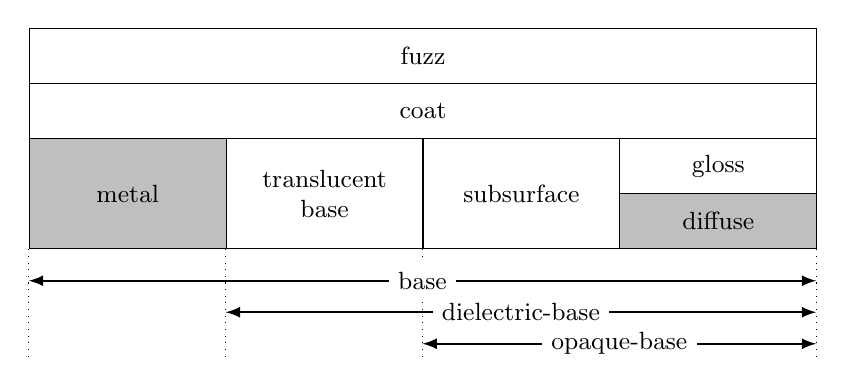
\begin{tikzpicture}[
      every node/.style={font=\small},
      layer/.style={draw, minimum height=1.4cm, minimum width=2.5cm, anchor=south west, text width=2cm, align=center},
      mid/.style={draw, minimum height=0.7cm, minimum width=2.5cm, anchor=south west, align=center},
      thin/.style={draw, minimum height=0.7cm, anchor=south west, minimum width=10cm, align=center},
    ]

    \draw[dotted] (0,1) -- (0,-0.4);
    \draw[dotted] (2.5,1) -- (2.5,-0.4);
    \draw[dotted] (5,1) -- (5,-0.4);
    \draw[dotted] (10,1) -- (10,-0.4);

    \node[layer, fill=lightgray] (metal) at (0,1) {metal};
    \node[layer] (translucent) at (2.5,1) {translucent base};
    \node[layer] (subsurface) at (5,1) {subsurface};
    \node[mid] (gloss) at (7.5,1.7) {gloss};
    \node[mid, fill=lightgray] (diffuse) at (7.5,1) {diffuse};

    \node[thin] (fuzz) at (0,3.1) {fuzz};
    \node[thin] (coat) at (0,2.4) {coat};

    \draw[>=latex,thick,<->] (0,0.6) -- (10,0.6) node[midway, fill=white] {base};
    \draw[>=latex,thick,<->] (5,-0.2) -- (10,-0.2) node[midway, fill=white] {opaque-base};
    \draw[>=latex,thick,<->] (2.5,0.2) -- (10,0.2) node[midway, fill=white] {dielectric-base};


  \end{tikzpicture}
  \caption{The different layers of the \gls{OpenPBR} surface shading model. The workflow supports various features such as metallic, glossy, and diffuse reflection renderings that are important for industrial use cases.}
  \label{fig:openPBR}
\end{figure}

% todo: consider re-integrating, but probably should contain a bit more references such as ggx…
% Diffuse reflection is based on the Oren-Nayar reflection model which extended the Lambertian model to include rough surfaces \cite{oren1994generalization}.

\subsubsection{Assessment}

While there is a large variety of material description standards, \gls{OpenPBR} is a promising candidate. The focus on surface shading is well-suited for the use case of this thesis. In comparison to other standards, it has significant industry backing, being adopted by major parties in the computer graphics industry such as Adobe, Autodesk and NVIDIA. Its design principles such as focusing on physical aspects, not specifying implementation details, and the \gls{uber shader} approach make it well-suited for real-time rendering.
